\section{Experimental Results}\label{sec:results}

We now present our experimental results: websites used (Sec.~\ref{subsection:dataset_characteristics}), poor search engine performance for this task (Sec.~\ref{subsubsection:search_engines}), baselines (Sec.~\ref{subsection:baselines}), crawling setup (Sec.~\ref{sec:exp-crawl-modalities}),
comparison of our crawler to baselines (Sec.~\ref{subsubsection:main_result}), and impact of hyper-parameters (Sec.~\ref{subsubsection:metaparameters_result}). Sec.~\ref{sec:exp-sb-algo} examines our Sleeping Bandit (SB) algorithm's effectiveness in grouping links into coherent and reward-based groups, and Sec.~\ref{sec:early_stopping} presents an early stopping mechanism.

\subsection{Websites}\label{subsection:dataset_characteristics}


\begin{table*}
	\caption{Main characteristics of websites (see detailed crawling methodology in Sec.~\ref{sec:exp-crawl-modalities})}
	%\vspace{-.5em}%\tiny
	%\hspace*{-3.75em}
  \begin{tabular}{cl@{}ccc@{\hspace{.75em}}c@{\hspace{.75em}}ccccc}
		\toprule
		          & \bfseries Starting URL                                & \bfseries Mlg.       & \bfseries F. C.  & \bfseries \#Available (k)                             &
    \bfseries \#Target (k) & \bfseries HTML to T. (\%) & \bfseries
    Target Size (MB) & \bfseries Target Depth                                                            \\
		\midrule
		\emph{ab} & \tiny\url{https://www.abs.gov.au/}                    & \xmark               & \xmark                        & 952.26                       & 263.26               & \08.86 & \04.50 ($\pm$\056.04)  & \0\08.94 ($\pm$\02.56) \\
		\emph{as} & \tiny\url{https://www.assemblee-nationale.fr/}        & \xmark               & \xmark                        & 949.42                       & 155.94               & \04.34 & \00.54 ($\pm$\0\06.38) & \0\05.84 ($\pm$\01.07) \\
		\emph{be} & \tiny\url{https://www.bea.gov/}                       & \xmark               & \cmark                        & \031.23                      & \015.84              & 32.19  & \02.03 ($\pm$\0\06.99) & \0\05.73 ($\pm$\03.21) \\
		\emph{ce} & \tiny\url{https://www.census.gov/}                    & \xmark               & \xmark                        & 988.37                       & 257.68               & \03.47 & \01.51 ($\pm$\015.77)  & \0\04.23 ($\pm$\00.48) \\
		\emph{cl} & \tiny\url{https://www.collectivites-locales.gouv.fr/} & \xmark               & \cmark                        & \0\05.54                     & \0\03.70             & \05.40 & \01.15 ($\pm$\0\04.91) & \0\02.80 ($\pm$\00.82) \\
		\emph{cn} & \tiny\url{https://www.cnis.fr/}                       & \xmark               & \cmark                        & \012.80                      & \0\07.49             & 13.87  & \00.43 ($\pm$\0\01.74) & \0\04.26 ($\pm$\01.59) \\
		\emph{ed} & \tiny\url{https://www.education.gouv.fr/}             & \xmark               & \cmark                        & 102.71                       & \010.47              & \03.95 & \01.00 ($\pm$\0\03.07) & \011.89 ($\pm$13.22)   \\
		\emph{il} & \tiny\url{https://www.ilo.org/}                       & \cmark               & \xmark                        & 990.71                       & \081.01              & \02.53 & 13.40 ($\pm$110.01)    & \0\04.26 ($\pm$\01.28) \\
		\emph{in} & \tiny\url{https://www.interieur.gouv.fr/}             & \xmark               & \cmark                        & 922.46                       & \022.98              & \01.54 & \01.12 ($\pm$\0\03.06) & \066.94 ($\pm$39.43)   \\
		\emph{is} & \tiny\url{https://www.insee.fr/}                      & \cmark               & \cmark                        & 285.55                       & 168.88               & 41.34  & \03.13 ($\pm$\021.43)  & \0\05.20 ($\pm$\01.81) \\
		\emph{jp} & \tiny\url{https://www.soumu.go.jp/}                   & \cmark               & \xmark                        & 993.87                       & 328.83               & \06.30 & \00.80 ($\pm$\0\04.49) & \0\05.18 ($\pm$\01.29) \\
		\emph{ju} & \tiny\url{https://www.justice.gouv.fr/}               & \xmark               & \cmark                        & \056.61                      & \014.85              & \04.85 & \00.48 ($\pm$\0\01.34) & \086.91 ($\pm$86.30)   \\
		\emph{nc} & \tiny\url{https://nces.ed.gov/}                       & \xmark               & \cmark                        & 309.97                       & \084.94              & 18.87  & \01.10 ($\pm$\011.56)  & \0\03.63 ($\pm$\01.66) \\
		\emph{oe} & \tiny\url{https://www.oecd.org/}                      & \cmark               & \cmark                        & 222.58                       & \045.04              & 15.61  & \02.31 ($\pm$\023.37)  & \0\06.28 ($\pm$\05.65) \\
		\emph{ok} & \tiny\url{https://okfn.org/}                          & \cmark               & \cmark                        & 423.12                       & \012.95              & \00.74 & \00.04 ($\pm$\0\00.24) & \0\02.64 ($\pm$\02.89) \\
		\emph{qa} & \tiny\url{https://www.psa.gov.qa/}                    & \cmark               & \cmark                        & \0\04.36                     & \0\02.45             & \04.15 & \02.97 ($\pm$\019.28)  & \0\03.03 ($\pm$\00.61) \\
		\emph{wh} & \tiny\url{https://www.who.int/}                       & \cmark               & \xmark                        & 351.86                       & \055.59              & 14.19  & \01.26 ($\pm$\011.14)  & \0\04.43 ($\pm$\00.62) \\
		\emph{wo} & \tiny\url{https://www.worldbank.org/}                 & \cmark               & \xmark                        & 223.67                       & \023.10              & \02.38 & \02.80 ($\pm$\027.16)  & \0\04.52 ($\pm$\00.69) \\
		\bottomrule
	\end{tabular}
	\label{tab:websites_characteristics}
\end{table*}

\def\websites{{as},{cl},{cn},{ed},{il},{in},{jp},{ju},{qa}}

Table~\ref{tab:websites_characteristics} lists the 18 websites used in our experiments.
As our primary application is a collaboration with French journalists~\cite{DBLP:conf/cikm/BalalauEGMMDGKP22} from \href{https://www.radiofrance.fr/}{RadioFrance},
six websites are French, public, and governmental: the \href{https://www.assemblee-nationale.fr/}{French National Assembly} (\emph{as}), \href{https://www.collectivites-locales.gouv.fr/}{French Local Communities} (\emph{cl}), \href{https://www.cnis.fr/}{French Council for Statistical Information} (\emph{cn}), and the ministries of \href{https://www.interieur.gouv.fr/}{Interior} (\emph{in}), \href{https://www.education.gouv.fr/}{Education} (\emph{ed}), and \href{https://www.justice.gouv.fr/}{Justice} (\emph{ju}). Each contains material on government branches, including SDs (our crawler's targets).
We also include eight multilingual websites: the UN's \href{https://www.ilo.org/}{International Labor Organization} (\emph{il}), \href{https://www.insee.fr/}{French Official Statistical Institute} (\emph{is}), \href{https://www.soumu.go.jp/}{Japan's Ministry of Interior} (\emph{jp}), \href{https://www.oecd.org/}{OECD} (\emph{oe}), \href{https://okfn.org/}{Open Knowledge Foundation} (\emph{ok}), \href{https://www.psa.gov.qa/}{Qatar's Official Statistical Service} (\emph{qa}), the UN \href{https://www.who.int/}{World Health Organization} (\emph{wh}), and the \href{https://www.worldbank.org/}{World Bank} (\emph{wo}).
Finally, we add national websites in English: the \href{https://www.abs.gov.au/}{Australian Bureau of Statistics} (\emph{ab}), \href{https://nces.ed.gov/}{US National Center for Education Statistics} (\emph{nc}), the \href{https://www.census.gov/}{US Census} (\emph{ce}), and the \href{https://www.bea.gov/}{US Bureau of Economic Analysis} (\emph{be}). Websites  in at least two languages have a \cmark{} in the ``\textbf{Mlg.}'' column.
The websites range from a few thousand to over 1M pages, excluding those resulting in 4xx or 5xx HTTP errors (see ``\textbf{\#Available (k)}'' column). A \xmark{} in the ``\textbf{F. C.}'' (``Fully Crawled'') column indicates incomplete crawls (Sec.~\ref{sec:exp-crawl-modalities}).

The following metrics assess the \emph{difficulty} and \emph{interest} of a focused crawl. For partially crawled websites, metrics are computed on the BFS-visited subset (Sec.~\ref{sec:exp-crawl-modalities}). ``\textbf{\#Target~(k)}'' is the total number of identified targets, and the ratio $\frac{\textrm{\#Target (k)}}{\textrm{\#Available (k)}}$ measures \emph{target density}; extremes are 66.78\% (\emph{cl}) and 2.49\% (\emph{in}). ``\textbf{HTML to T. (\%)}'' is the percentage of HTML pages linking to at least one target, reflecting the \emph{density of target-pointing pages} (e.g., \emph{cl} has the highest density, but all targets are concentrated in 5.40\% of HTML pages). ``\textbf{Target Size (MB)}'' gives the mean and standard deviation (STD) of target file sizes, and ``\textbf{Target Depth}'' the mean and STD of depths (shortest link navigation from the root). \emph{Mean depths vary greatly, from 3 to nearly 90}: highest values arise on portals requiring page-to-page navigation, e.g. \emph{ju}.
Table~\ref{tab:websites_characteristics} shows our websites are \emph{extremely diverse}: small or huge, varying in depth, target number and  locations, and over 20 languages. This diversity demands \emph{adaptable crawling strategies} to efficiently retrieve targets. A manual analysis of typical target locations on \emph{ju}, \emph{il}, \emph{wh}, and \emph{nc} is provided in the extended version in~\cite{github_repository}.


\begin{toappendix}

\subsection{Websites}

To further emphasize the diversity of crawling efforts, we manually analyzed the types of pages where targets are typically found. In \emph{ju}, targets appear under various resource lists and data portals disseminated across the website. Some are huge (e.g., \url{https://www.justice.gouv.fr/documentation/bulletin-officiel}), while others are smaller (e.g., \url{https://www.justice.gouv.fr/documentation/ressources/conventions-judiciaires-dinteret-public}). Some require multi-step navigation to reach deeper pages that contain one or a few target links. In \emph{il}, most targets are found in small, dispersed data catalogs: some gathered in ``ILOSTAT'' (\url{https://ilostat.ilo.org/}), others accessible only through further exploration. These targets are generally downloadable directly from the catalogs. In \emph{wh}, the majority of targets require multi-step navigation through a hierarchy of subjects and sub-subjects, with only a subset leading to targets: efficient crawling thus requires quickly identifying interesting parts. In \emph{nc}, all previously mentioned typologies are present: data portals (e.g., \url{https://nces.ed.gov/national-center-education-statistics-nces/products}), exhaustive lists (e.g., \url{https://nces.ed.gov/surveys/spp/results.asp}), and deep pages requiring multi-step navigation.
\end{toappendix}

\subsection{Search Engines and Dataset Search}
\label{subsubsection:search_engines}

We attempted to retrieve SDs using search engines (SEs), in particular by testing three popular Google services:
\href{https://www.google.com/}{classical search} (GS), \href{https://datasetsearch.research.google.com/}{Google Datasets Search} (GDS), and the \href{https://www.google.com/publicdata/directory}{Google Public Data Explorer} (GPDE) providing data from international
organizations.

GS allows filtering by website (\textsf{\small site:}) and file type (\textsf{\small filetype:}), via its Web interface and \href{https://programmablesearchengine.google.com/}{API}. However, SEs, including Google, do not fully index websites and GS caps results at 1k, often truncating them. 
For instance, querying \emph{ju} for PDFs yields only 302 results, although more than 9k exist; similarly, only 240 ODS files are returned (out of 910), and on \emph{in} 38 XLS (out of 1\,546). Even worse: TSV is not recognized at all despite 11\,097 files on \emph{ju}. On \emph{il}, GS lists 641 results instead of over 49k, and no ZIP archives instead of at least 2\,239.
GDS trims results even further, e.g., 109 tabular files on
\emph{ju} (vs. 1\,188); 93 datasets on \emph{il} (vs.\ $\geq$170k found by our crawler); and 312 on \emph{ce} (vs.\ 800k), etc. 
GPDE is built for human readers, indexing from a closed, fixed set of providers, such as \href{https://ec.europa.eu/eurostat/}{Eurostat}, \emph{wo}, \href{https://www.statcan.gc.ca/}{Statistics Canada}, and \emph{oe}, but excludes key sites like UN’s \emph{wh}, \emph{il}, and US agencies (\emph{be}, \emph{nc}, \emph{ce}).	
GPDE only allows manual exploration, plotting datasets guided by users' filters but offering neither downloads nor links to originals: e.g., it displays 150 OECD statistics across 37 countries and 100 years, but only references a 272-page PDF (\href{https://www.oecd-ilibrary.org/}{OECD iLibrary}).  


Overall, \textbf{SEs lack transparency and control over the retrieved SDs}, a critical limitation for our task. In contrast, our crawler retrieves all data files within a specified budget, with explainable decisions and explicit choice of target MIME types.
\subsection{Baselines}
\label{subsection:baselines}

We compare our best-performing \textsf{\small SB-CLASSIFIER} with an adapted version in which the URL classifier is replaced by an (unrealistic) perfect oracle~(\textsf{\small SB-ORACLE}), as well as with several baseline methods. First, we consider four simple crawlers.
\begin{inparaenum}[(i)]
\item The \textsf{\small RANDOM} crawler selects the next hyperlink to visit
	uniformly at random from the crawl frontier.
	\item The
    \emph{Breadth-First Search} (\textsf{\small BFS}) exhaustive crawler maintains the
	frontier as a \emph{First-In-First-Out queue} data structure. It crawls
	all pages reachable by a path of length $\ell$ before any page reachable
	only by longer paths ($\ell' > \ell$).
	\item \emph{Depth-First
    Search} (\textsf{\small{DFS}}) maintains the frontier in a \emph{Last-In-First-Out stack}.
	It is rarely used for exhaustive crawling since it may fall
        into
	\href{https://en.wikipedia.org/wiki/Spider_trap}{robot traps}.
	\item The unrealistic \emph{Omniscient Crawler} (\textsf{\small OMNISCIENT}) knows all target URLs ($V^*$) from the start and crawls them sequentially. Since an optimal crawler is intractable (Prop.~\ref{prop:np-complete}), this omniscient crawler provides an (unreachable) upper bound on crawler efficiency.
\end{inparaenum}


The \emph{Offline-Trained, Tag Path-Based Crawler} (\textsf{\small TP-OFF})~\cite{faheem2015adaptive} is a closely related focused crawler originally designed to retrieve \emph{diverse} textual content. We apply it \emph{technically unchanged}, except for redefining its reward to target retrieval.
As described in~\cite{faheem2015adaptive}, it first crawls 3k pages with BFS and groups the tag paths leading to followed links as in Sec.~\ref{subsection:states_actions}. Page benefits are computed immediately, and tag path groups are stored in a priority queue ordered by average benefit. After these 3k pages, \cite{faheem2015adaptive} \emph{only considers links matching existing tag path groups} (ordered by priority), other are ignored. 
In our context, benefit computation requires knowing if links lead to targets. To enable this baseline, \emph{we provide it with the true benefit} (number of targets behind a page's links) as if given by an oracle, for the initial 3k pages. Beyond this point, newly formed tag path groups receive a fixed benefit of~0. This baseline, given an unfair advantage in its first stage, can be seen as an \emph{ablated} version of ours, learning \emph{offline} instead of \emph{online} with our RL method.

The \emph{Focused Crawler} (\textsf{\small FOCUSED}) represents early generic focused crawling approaches that rely on a classifier to estimate the likelihood that a newly discovered hyperlink leads to a target~\cite{chakrabarti1999focused,diligenti2000focused}. The frontier is maintained as a \emph{priority queue},  favoring links predicted to be relevant. It relies on a standard \emph{logistic regression}, periodically retrained on crawled pages at no extra HTTP cost.
Its features follow standard focused crawler practice: the (approximated) depth of the source page, a 2-gram BoW representation of the URL (similarly to Sec.~\ref{subsection:url_classifier}), and a 2-gram BoW representation of the link's \emph{anchor} text~\cite{chakrabarti1999focused,diligenti2000focused}. \emph{Topic-oriented} features are intentionally excluded (further discussed in Sec.~\ref{section:related_work}). Overall, \textsf{\small FOCUSED} can be viewed as an \emph{ablated} version of our crawler, as it neither exploits tag-path structure (Sec.~\ref{subsection:url_classifier}) nor uses RL (Sec.~\ref{subsection:crawling_algorithm}).


{\textsf{\small TRES}}~\cite{kontogiannis2022tree} is a topical, RL-based focused crawler using a Bi-LSTM classifier to assess HTML page relevance. Like our approach, it employs RL to learn where interesting content resides in a website. However, {\textsf{\small TRES}} defines interestingness through a user-specified topic, whereas we target SDs regardless of subject. As it targets topic-relevant HTML pages only, it requires input keywords, positive HTML examples, and is limited to one language.
To include {\textsf{\small TRES}} as a baseline for SD retrieval, we made changes related to its focus, \emph{without altering its core logic or technical components}. Specifically, we give it three \emph{unfair advantages}: \begin{inparaenum}[(i)]
\item \textsf{\small TRES} expects a list of topic-specific keywords to initialize its classifier's training: we supply 74 hand-crafted terms likely to appear in links' anchors to targets to initialize its classifier.  
\item We provide 1k HTML pages with links to targets from the evaluation websites as positive examples (based on prior crawls), as required to pre-train its classifier, giving it partial access to the solution.  
\item \textsf{\small TRES} must classify URLs as HTML or not to manage its frontier, as it only accepts HTML pages. Although costly in practice (see Sec.~\ref{subsection:url_classifier}), we gave it an oracle doing this classification at no cost, giving it its chance while not affecting its original behavior.
\end{inparaenum}
Since its RL agent and classifier rely only on textual HTML features, {\textsf{\small TRES}} cannot directly detect targets. We therefore added two adjustments: links are added to the frontier as in~\cite{kontogiannis2022tree}, while others (which TRES would normally ignore) are visited immediately and targets counted if found; and its language filter was disabled, preventing coarse URL-based false exclusions. The modified code is available at~\cite{tres_modified_repository}.

\begin{toappendix}
  \subsection{Baselines}
    We use the following list of keywords as initial input to
  \textsf{\small TRES} to train its classifier:
    \begin{multicols}{4}
      \noindent
      pdf\\
xls\\
csv\\
tar\\
zip\\
rar\\
rdf\\
json\\
doc\\
xml\\
yaml\\
txt\\
tsv\\
ppt\\
ods\\
dta\\
7z\\
ttl\\
file\\
document\\
report\\
publication\\
dataset\\
data\\
download\\
archive\\
spreadsheet\\
table\\
list\\
resource\\
annex\\
supplement\\
attachment\\
proceedings\\
survey\\
material\\
output\\
content\\
statistics\\
article\\
paper\\
metadata\\
fact\\
download file\\
download document\\
available for download\\
access data\\
view report\\
get dataset\\
data file\\
read more\\
resource list\\
get document\\
download pulication\\
document archive\\
supporting materials\\
export data\\
download CSV\\
download PDF\\
download XLS\\
dataset download\\
attached document\\
official documents\\
browse files\\
download statistics\\
download article\\
annual report\\
white paper\\
technical documentation\\
technical report\\
raw data\\
metadata file\\
open data\\
fact sheet\\

    \end{multicols}
  
\end{toappendix}

\subsection{Practical Crawling in our Experiments}
\label{sec:exp-crawl-modalities}

To evaluate six baselines and our crawler with various
hyper-parameters, repeated crawls per website are infeasible
due to time constraints (e.g., large files or slow connections), and crawling ethics. Thus, for each website, all baselines and our crawler run in a setting where \emph{each first checks if the resource is already stored in a local database}. If so, we use it; otherwise, we fetch it via HTTP~GET and the URL, HTTP status, headers, and response body are stored.

\emph{For evaluation purposes only}, we stop crawling a website under any of the following conditions:
\begin{inparaenum}[(i)]
	\item One crawler terminates before reaching 1M pages, yielding a complete local replication: all others then rely solely on database look-ups.
	\item All crawlers reach 1M visited webpages (possibly not the
          same pages across crawlers).
    \item A 3-week time limit is reached, as crawling can be extremely slow for some websites (across 18 sites, 22.2M distinct pages were retrieved).
	\item A crawler exceeds 1 minute between two requests, excluding network latency (only affecting \textsf{\small TRES}).
\end{inparaenum}

We conduct and present our experiments as follows:
\begin{inparaenum}[(i)]
    \item We carry hyper-parameter studies and evaluate our URL classifier on fully-crawled websites with \emph{fewer than 1M pages}. Full replication enables parallel runs under multiple parameter settings and provides complete knowledge for both (unrealistic) \textsf{\small SB-ORACLE} crawler and \textsf{\small TRES} baseline (see Sec.~\ref{subsubsection:main_result}).
	\item On websites where \emph{all baselines reach 1M webpages}, crawlers are compared on the subset of the website each of them visited. Note that their target sets, and the retrieved data volume, may differ: a good crawler prioritizes \emph{more target-rich} pages.
    \item On websites where \emph{at least one baseline did not crawl 1M pages within the time limit}, crawlers are compared on the smallest crawl size achieved: e.g., if three crawlers visit 400k, 200k, and 800k pages, respectively, we compare them on their first 200k pages.
    \item On websites where \emph{at least one baseline fails to reach 1M pages} within the time limit, crawlers are compared on the smallest crawl size achieved: e.g., if crawlers visit 400k, 200k, and 800k pages, results are computed on their first 200k pages.

\end{inparaenum}

We
exclude retrieval times from our results, 
since these vary out of our control. 
We focus on the \emph{number of requests and data volumes}; crawl time
can be estimated from these, knowing the bandwidth and the ethics waiting
time. To illustrate retrieval times, on the medium-sized website
\emph{ed}, \textsf{\small SB-CLASSIFIER} requires 3h~16min to collect 5k
targets and 10h~52min to collect 10k, whereas \textsf{\small BFS} requires
5h~13min and 48h~45min respectively (1.6$\times$ and 4.5$\times$ more).

\subsection{Comparison with Baselines}\label{subsubsection:main_result}

\begin{toappendix}
  \subsection{Comparison with Baselines}

In the experiments, we apply filters on MIME types and URL
extensions to avoid downloading multimedia content. The MIME types in the
blocklist are those for multimedia content, namely \texttt{image/*},
\texttt{audio/*}, and \texttt{video/*}. The associated URL extensions are
the following:

{\small\ttfamily
\begin{multicols}{12}
\noindent
.3g2\\
.3ga\\
.3gp2\\
.3gp\\
.3gpa\\
.3gpp2\\
.3gpp\\
.aac\\
.aacp\\
.adp\\
.aff\\
.aif\\
.aiff\\
.arw\\
.asf\\
.asx\\
.avi\\
.avif\\
.avifs\\
.bmp\\
.btif\\
.cgm\\
.cmx\\
.cr2\\
.crw\\
.dcr\\
.djv\\
.djvu\\
.dng\\
.dts\\
.dtshd\\
.dwg\\
.dxf\\
.ecelp4800\\
.ecelp7470\\
.ecelp9600\\
.eol\\
.erf\\
.f4v\\
.fbs\\
.fh4\\
.fh5\\
.fh7\\
.fh\\
.fhc\\
.flac\\
.fli\\
.flv\\
.fpx\\
.fst\\
.fvt\\
.g3\\
.gif\\
.h261\\
.h263\\
.h264\\
.heic\\
.heif\\
.icns\\
.ico\\
.ief\\
.jfi\\
.jfif-tbnl\\
.jfif\\
.jif\\
.jpe\\
.jpeg\\
.jpg\\
.jpgm\\
.jpgv\\
.jpm\\
.k25\\
.kar\\
.kdc\\
.lvp\\
.m1v\\
.m2a\\
.m2v\\
.m3a\\
.m3u\\
.m4a\\
.m4b\\
.m4p\\
.m4r\\
.m4u\\
.m4v\\
.mdi\\
.mid\\
.midi\\
.mj2\\
.mjp2\\
.mka\\
.mkv\\
.mmr\\
.mov\\
.movie\\
.mp2\\
.mp2a\\
.mp3\\
.mp4\\
.mp4v\\
.mpa\\
.mpe\\
.mpeg\\
.mpg4\\
.mpg\\
.mpga\\
.mrw\\
.mxu\\
.nef\\
.npx\\
.oga\\
.ogg\\
.ogv\\
.opus\\
.orf\\
.pbm\\
.pct\\
.pcx\\
.pef\\
.pgm\\
.pic\\
.pjpg\\
.png\\
.pnm\\
.ppm\\
.psd\\
.ptx\\
.pya\\
.pyv\\
.qt\\
.ra\\
.raf\\
.ram\\
.ras\\
.raw\\
.rgb\\
.rlc\\
.rmi\\
.rmp\\
.rw2\\
.rwl\\
.snd\\
.spx\\
.sr2\\
.srf\\
.svg\\
.svgz\\
.tif\\
.tiff\\
.ts\\
.viv\\
.wav\\
.wax\\
.wbmp\\
.weba\\
.webm\\
.webp\\
.wm\\
.wma\\
.wmv\\
.wmx\\
.wvx\\
.x3f\\
.xbm\\
.xif\\
.xpm\\
.xwd\\

\end{multicols}}

Note that URL extension filters are not useful on all websites (on some,
URLs don't usually include any extension, see the discussion at the
beginning of Section~\ref{subsection:url_classifier}).
\end{toappendix}

\begin{figure*}
	\captionsetup[subfigure]{labelformat=simple, labelsep=period}
    \renewcommand{\thesubfigure}{\arabic{subfigure}}
	\begin{subfigure}[t]{\textwidth}
		
\includegraphics[width=\linewidth]{plots/oracle_vs_classifier/legend.pdf}
	\end{subfigure}
	\foreach \i [count=\n from 1] in \websitesSinglePage {
		\begin{subfigure}[t]{0.47\textwidth}
			\includegraphics[width=\linewidth]{plots/oracle_vs_classifier/\i.pdf}

			\vspace{-1em}
			\caption{\getfullname{\n}}
		\end{subfigure}
		\qquad
	}

	\vspace{-.75em}
  \caption{Comparison of different crawler performance for 10
    selected websites presented in
Table~\ref{tab:websites_characteristics}; for {\small TRES}, experiments
are only shown for fully-crawled websites. {\small SB-CLASSIFIER} is the proposed approach.}
	\label{fig:10_sites_plots}
\end{figure*}


\begin{table*}
	\centering
	\caption{Percentage of requests that each crawler performs to retrieve 90\% of the targets, for websites in Table~\ref{tab:websites_characteristics}. Below double horizontal rule, percentage of saved requests and percentage of lost targets due to early-stopping mechanism (see Sec.~\ref{sec:early_stopping}).}

	\setlength{\tabcolsep}{3pt}
	\begin{tabular*}{\textwidth}{@{\extracolsep{\fill}}r*{18}{c}}
		\toprule
		\bfseries \diagbox{\scriptsize Crawler}{\scriptsize Website}         & {\emph{ab}}     & {\emph{as}}     & {\emph{be}}     & {\emph{ce}}     & {\emph{cl}}     & {\emph{cn}}     & {\emph{ed}}     & {\emph{il}}     & {\emph{in}}     & {\emph{is}}     & {\emph{jp}}     & {\emph{ju}}     & {\emph{nc}}     & {\emph{oe}}     & {\emph{ok}}     & {\emph{qa}}     & {\emph{wh}}     & {\emph{wo}}     \\
		\midrule
		\textsf{\small SB-ORACLE} & {NA}            & {NA}            & {72.6}          & {NA}            & {70.7}          & {70.3}          & {48.0}          & {NA}            & {12.8}          & {73.8}          & {NA}            & {34.1}          & {50.8}         & {55.8}          & {13.8}          & {47.3}          & {NA}            & {NA}            \\
		\textsf{\small SB-CLASS.} & {\textbf{31.2}} & {\textbf{35.1}} & {\textbf{75.7}} & {\textbf{23.5}} & {74.4} & {\textbf{70.9}} & {\textbf{51.5}} & {\textbf{14.2}} & {\textbf{11.9}} & {\textbf{76.0}} & {\textbf{37.7}} & {\textbf{35.8}} & {\textbf{51.6}} & {\textbf{59.2}} & {\textbf{15.5}} & {\textbf{57.7}} & {\textbf{19.7}} & {\textbf{18.6}} \\
		\midrule
		\textsf{\small FOCUSED}   & {68.2}          & {$+\infty$}     & {87.8}          & {36.0}          & {88.9}          & {82.7}          & {86.7}          & {$+\infty$}     & {62.8}          & {86.9}          & {42.0}         & {91.1}          & {92.8}          & {84.9}          & {51.8}          & {71.0}          & {$+\infty$}     & {$+\infty$}     \\
		\textsf{\small TP-OFF}    & {96.4}          & {50.3}          & {86.2}          & {34.7}          & {81.8}          & {88.2}          & {95.6}          & {$+\infty$}     & {99.7}          & {88.0}          & {$+\infty$}     & {74.4}          & {93.0}          & {88.7}          & {76.2}          & {88.6}          & {$+\infty$}     & {$+\infty$}     \\
		\textsf{\small BFS}       & {97.4}          & {90.8}          & {89.1}          & {73.5}          & {87.5}         & {80.0}          & {94.6}          & {33.2}          & {99.3}          & {92.7}          & {45.2}          & {80.8}          & {81.8}         & {96.5}          & {66.8}          & {70.6}          & {79.0}          & {92.0}          \\
		\textsf{\small DFS}       & {83.7}          & {$+\infty$}     & {85.2}          & {74.9}          & {\textbf{70.6}} & {84.6}          & {90.5}          & {$+\infty$}     & {99.7}          & {87.7}          & {45.6}          & {80.2}          & {93.7}          & {88.7}          & {80.5}          & {74.4}          & {$+\infty$}     & {$+\infty$}     \\
		\textsf{\small RANDOM}    & {$+\infty$}     & {98.2}          & {92.4}          & {44.5}          & {89.2}          & {85.1}          & {95.0}          & {$+\infty$}     & {99.0}          & {92.7}          & {$+\infty$}     & {83.2}          & {87.9}          & {96.8}          & {85.0}          & {77.8}          & {71.0}          & {$+\infty$}     \\
		\midrule
    \addlinespace[-0.2ex]
		\midrule
		{Saved req.} & {34.4} & {\00.0} & {\00.0} & {\00.0} & {\00.0} & {\00.0} & {27.4} & {\00.0} & {82.6} & {\02.2} & {39.0} & {18.8} & {20.4} & {\00.0} & {73.1} & {\00.0} & {\00.0} & {\00.0} \\
		{Lost targets} & {13.5} & {\00.0} & {\00.0} & {\00.0} & {\00.0} & {\00.0} & {\00.1} & {\00.0} & {\00.0} & {\00.0} & {\02.5} & {\00.4} & {\00.1} & {\00.0} & {\02.0} & {\00.0} & {\00.0} & {\00.0} \\
		\bottomrule
	\end{tabular*}
	\label{tab:all_crawlers_all_sites_nb_requests}
\end{table*}

\begin{toappendix}
  \bigskip

	\def\websitesAppendix{{ab}, {as}, {be}, {cn}, {is}, {jp}, {oe}, {qa}}

	\begin{figure*}[b]
	\captionsetup[subfigure]{labelformat=simple, labelsep=period}
    \renewcommand{\thesubfigure}{\arabic{subfigure}}
		\begin{subfigure}[t]{\textwidth}
			
\includegraphics[width=\linewidth]{plots/oracle_vs_classifier/legend.pdf}
		\end{subfigure}
		\foreach \short in \websitesAppendix {
			\begin{subfigure}[t]{0.47\textwidth}
				\includegraphics[width=\linewidth]{plots/oracle_vs_classifier/\short.pdf}

				\vspace{-1em}
				\caption{\emph{\short}}
			\end{subfigure}
			\qquad
		}

		\caption{Comparison of different crawler performance for the 8 websites not presented in Figure~\ref{fig:10_sites_plots} due to space reasons;
for {\small TRES}, experiments
are only shown for fully-crawled websites}
		\label{fig:8_last_sites_plots}
	\end{figure*}
	Figure~\ref{fig:8_last_sites_plots} completes
  Figure~\ref{fig:10_sites_plots} with the eight remaining websites plots
  that could not fit in the paper (see
  Table~\ref{tab:websites_characteristics} for characteristics of
  websites). Figures~\ref{fig:hyper_param_alpha_1} to \ref{fig:hyper_param_similarity_threshold_2} present exhaustive graphical results of the hyper-parameters studies conducted on the 11 fully-crawled websites. Especially, Figures~\ref{fig:hyper_param_alpha_1} and \ref{fig:hyper_param_alpha_2} study the exploration--exploitation coefficient $\alpha$, Figures~\ref{fig:hyper_param_n_grams_1} and \ref{fig:hyper_param_n_grams_2} study the choice of $n$ in $n$-grams used in tag paths vector representation, and  Figures~\ref{fig:hyper_param_similarity_threshold_1} and \ref{fig:hyper_param_similarity_threshold_2} study the similarity threshold $\theta$.
\end{toappendix}

\begin{table*}
	\centering
	\caption{Fraction of non-target volume each crawler retrieves before reaching 90\% of total target volume, for websites in Table~\ref{tab:websites_characteristics}}.

	\setlength{\tabcolsep}{3pt}
	\begin{tabular*}{\textwidth}{@{\extracolsep{\fill}}r*{18}{c}}
		\toprule
		\bfseries  \diagbox{\scriptsize Crawler}{\scriptsize Website}         & {\emph{ab}}    & {\emph{as}}     & {\emph{be}}     & {\emph{ce}}     & {\emph{cl}}     & {\emph{cn}}     & {\emph{ed}}     & {\emph{il}}      & {\emph{in}}     & {\emph{is}}     & {\emph{jp}}     & {\emph{ju}}     & {\emph{nc}}     & {\emph{oe}}     & {\emph{ok}}     & {\emph{qa}}     & {\emph{wh}}     & {\emph{wo}}     \\
		\midrule
		\textsf{\small SB-ORACLE} & {NA}            & {NA}            & {24.2}          & {NA}            & {56.3}          & {24.6}          & {49.2}          & {NA}             & {12.5}          & {59.7}          & {NA}            & {22.9}          & {29.5}          & {48.0}          & {33.2}          & {30.2}          & {NA}            & {NA}            \\
		\textsf{\small SB-CLASS.} & {\textbf{20.4}} & {\textbf{21.4}} & {\textbf{29.5}} & {\textbf{29.1}} & {56.0}          & {\textbf{29.0}} & {\textbf{49.2}} & {53.2}           & {\textbf{23.6}} & {\textbf{64.7}}          & {\textbf{18.6}} & {\textbf{23.1}} & {\textbf{34.5}} & {\textbf{49.5}} & {\textbf{34.9}} & {\textbf{33.2}} & {\textbf{32.7}} & {\textbf{35.8}} \\
		\midrule
		\textsf{\small FOCUSED}   & {$+\infty$}     & {$+\infty$}     & {85.2}          & {97.0}          & {76.3}          & {74.7}          & {86.4}          & {$+\infty$}      & {67.3}          & {73.8} & {66.8}          & {72.2}          & {84.9}          & {72.7}          & {49.8}          & {80.3}          & {$+\infty$}     & {$+\infty$}     \\
		\textsf{\small TP-OFF}    & {$+\infty$}     & {$+\infty$}     & {92.3}          & {64.4}          & {65.0}          & {94.7}          & {92.9}          & {$+\infty$}      & {98.8}          & {89.7}          & {$+\infty$}     & {72.3}          & {89.2}          & {89.0}          & {73.6}          & {46.9}          & {$+\infty$}     & {$+\infty$}     \\
		\textsf{\small BFS}       & {81.8}          & {75.7}          & {66.5}          & {98.5}          & {80.8}          & {50.4}          & {93.2}          & {\textbf{\03.6}} & {99.0}          & {93.8}          & {54.0}          & {68.0}          & {84.5}          & {97.5}          & {63.3}          & {87.3}          & {91.5}          & {98.3}          \\
		\textsf{\small DFS}       & {98.6}          & {$+\infty$}     & {64.2}          & {97.0}          & {\textbf{45.0}} & {82.4}          & {90.8}          & {$+\infty$}     & {98.1}          & {85.0}          & {59.5}          & {68.6}          & {96.1}          & {90.5}          & {97.0}          & {75.0}          & {$+\infty$}     & {$+\infty$}     \\
		\textsf{\small RANDOM}    & {71.6}          & {$+\infty$}     & {83.4}          & {$+\infty$}     & {89.3}          & {82.7}          & {92.9}          & {$+\infty$}      & {95.8}          & {98.3}          & {$+\infty$}     & {70.1}          & {88.2}          & {98.1}          & {86.6}          & {77.8}          & {$+\infty$}     & {$+\infty$}     \\
		\bottomrule
	\end{tabular*}
	\label{tab:all_crawlers_all_sites_volume}
\end{table*}

Figure~\ref{fig:10_sites_plots} compares our crawler's performance with the baselines on 10 diverse, representative websites; the other plots are in the extended version~\cite{github_repository}. Default settings are $n=2$ ($n$-grams), $\theta=0.75$, $\alpha=2\sqrt{2}$, $m=12$ (path vector dimension), $w=15$ (hash function), and $b=10$ (batch size). MIME type and extension blocklists are chosen to filter out multimedia content (image, audio, video), usually large in volume. Full lists are in~\cite{github_repository}. 

In addition, for each crawler and all 18 websites, Table~\ref{tab:all_crawlers_all_sites_nb_requests} (above the double rule) shows \emph{the percentage of requests needed to retrieve 90\% of targets}, and Table~\ref{tab:all_crawlers_all_sites_volume} \emph{the percentage of non-target page volume retrieved before reaching 90\% of total target volume}. Lower values indicate greater efficiency. For partially crawled sites, metrics are computed on pages visited by BFS.
 If a crawler never reaches the 90\%, we show $+\infty$.
The best-performing crawler per website is in bold, excluding \textsf{\small SB-ORACLE} (as unrealistic). 
 For each website in Figure~\ref{fig:10_sites_plots}, two graphs show crawler performance: on the left, the \emph{number of crawled targets v.s.\ number of HTTP requests} (both GET
and HEAD, in thousands); 
on the right, the \emph{volume of
	target responses (GB) v.s.\ volume of non-target ones}. In both
graphs, \emph{a higher curve is better}.

For \emph{fully-crawled websites},
we run two variants of our crawler:  \textsf{\small SB-CLASSIFIER} 
and \textsf{\small SB-ORACLE} (see Sec.~\ref{subsection:baselines}).
This assesses the impact of the URL classifier on crawl performance. 
Results are \emph{averaged over 15 runs}, with shaded areas indicating $\pm$ one STD. STD are in most cases low, indicating stable behavior. Variability arises mainly from: randomness in link selection within chosen actions; the stochastic SGD-trained classifier; and the single-state RL agent, whose design is crucial for stabilization (see~\cite{github_repository}).


For \emph{partially crawled websites}, we report a single run of \textsf{\small SB-CLASSIFIER}, lacking perfect classifier information, and since multiple crawls are unfeasible 
(Sec.~\ref{sec:exp-crawl-modalities}). All baselines but \textsf{\small RANDOM} and \textsf{\small TRES} are deterministic, thus one run suffices. \textsf{\small TRES} is only evaluated on the 10 smallest fully-crawled websites, as it requires oracle access and does not scale: beyond small websites (\emph{be}, \emph{cl}, \emph{cn}, and \emph{qa}), it exceeds the 1-minute-per-request threshold and is stopped before completing the crawl of larger websites. Crawling 100k additional pages at that point would require at the very least 10 more weeks.

The plots and Tables~\ref{tab:all_crawlers_all_sites_nb_requests} and \ref{tab:all_crawlers_all_sites_volume} show that \textbf{our crawler with the URL
classifier outperforms all baselines}, with one exception: on \emph{cl}, \textsf{\small DFS} is slightly better near the end. On \emph{il} (volume only) \textsf{\small BFS} briefly surpasses ours, but overall our crawler retrieves twice more targets.  
\textbf{For websites \emph{as}, \emph{ce}, \emph{ed}, \emph{il}, \emph{in}, \emph{ju}, \emph{nc}, \emph{wh}, and \emph{wo}, \textsf{\small SB-CLASSIFIER}} significantly reduces resource usage (time or bandwidth) to reach a fixed number of targets or maximize targets under a budget. 
On \emph{wo}, the best baseline (\textsf{\small BFS}) would require 3 months to match our targets (linear extrapolation), and \textsf{\small FOCUSED} 9 months; on \emph{wh}, the best baseline (\textsf{\small RANDOM}) would require 3 months and the worst (\textsf{\small TP-OFF}) 6 years. On \emph{il}, the top-3 baselines find no targets in the last 650k iterations, whereas ours continues until the end.


On other sites (\emph{be}, \emph{cn}, \emph{cl}, \emph{jp}, \emph{qa}), while some baselines approach \textsf{\small SB-CLASSIFIER} performance, it remains superior overall, outperforming all baselines on a wide variety of websites, with respect to the size, depth, target distribution, etc.
Small sites (\emph{be}, \emph{cl}, \emph{cn}, \emph{qa}) are traversed quickly, allowing less learning, yet our approach adapts effectively.  

\textsf{\small TP-OFF} performs poorly, especially on \emph{ed}, \emph{il}, \emph{jp}, \emph{wh}, and \emph{wo}.
Learning from just 3k pages proves insufficient on large websites. 
On \emph{cn}, \textsf{\small TP-OFF} underperforms BFS after the initial 3k pages, despite only three times more pages remaining. Increasing the training set could help but would approach the simplicity of a standard \textsf{\small BFS} crawler.
\textsf{\small FOCUSED} is outperformed by ours on all websites, showing early focused-crawlers are too basic to efficiently solve our problem.
On 10 websites out of 18, it is even beaten by \textsf{\small BFS}, \textsf{\small DFS} or \textsf{\small RANDOM}.

Despite being given three unfair advantages (hand-picked keywords, access to training pages with target links, and an oracle for URL type prediction), 
\textsf{\small TRES} fails on 9 out of 10 websites, performing reasonably only on \emph{oe} and only until it had to be stopped. More critically, \textsf{\small TRES} cannot scale to medium or large sites, even when run fully locally. Crawl iterations slow dramatically due to exhaustive feature-based evaluations during tree expansion.
These results confirm that topical crawlers are fundamentally ill-suited for direct target retrieval, even when heavily adapted and unfairly favored.

Comparing our \textsf{\small SB-CLASSIFIER} with \textsf{\small SB-ORACLE}
shows that our classifier is close to the (virtual)
	perfect oracle. Further analysis (our classifier's impact) is
  provided in the extended version~\cite{github_repository}.

\subsection{Hyper-Parameters}\label{subsubsection:metaparameters_result}

We present the impact of three key hyper-parameters ($\alpha$, $n$, and $\theta$) on crawl performance. Table~\ref{tab:parameter_study} reports the number of requests (resp. response volume for non-target pages) needed to retrieve 90\% of the targets (resp. target volume);
full plots are available in~\cite{github_repository}. When varying one parameter, others remain at default values (Sec.~\ref{subsubsection:main_result}). Additional parameters, including the projection dimension~$D$ (Sec.~\ref{subsection:group-links}), showed no significant effect.

\begin{inparaenum}
	\item \emph{Impact of $\alpha$.} $\alpha$ controls the exploration--exploitation trade-off (Sec.~\ref{subsection:group-links}). We test $\alpha \in \{0.1,2\sqrt{2},30\}$ (Table~\ref{tab:parameter_study}, top), as optimality of $2\sqrt{2}$ is not guaranteed in our non-standard MAB setting. Smaller $\alpha$ generally improves performance, with best results for $\alpha=2\sqrt{2}$. Large $\alpha$ leads to excessive \emph{exploration}, especially on low or moderate-reward websites, neglecting useful, already discovered actions.
	\item \emph{Impact of $n$ in $n$-grams for tag path representation.} For merging tag paths (Sec.~\ref{subsection:states_actions}), we test $n \in \{1,2,3\}$ ($n=1$ represents paths as sets of HTML tags). Table~\ref{tab:parameter_study} (middle) shows that $n=2$ and $3$ generally outperform $n=1$, confirming that groups of tag paths provide a better learning basis than sets of tags. We choose $n=2$, as $3$ yields similar performance but incurs higher computational cost due to exponential growth feature space growth.
	\item \emph{Impact of $\theta$.} The similarity threshold $\theta$ controls tag path grouping (Sec.~\ref{subsection:states_actions}). We test $\theta \in \{0.55,0.75,0.95\}$ (Table~\ref{tab:parameter_study}, bottom). High $\theta$ often performs poorly, especially when no similarity $>95\%$ exists, as with websites adding unique IDs in tags. For example, on \emph{ed} it caused an OOM error by creating as many actions as HTML pages. Best results occur with $\theta \in \{0.55,0.75\}$, with $\theta=0.75$ usually superior: when $0.55$ performs better, $0.75$ remains comparable, but not conversely (e.g., on \emph{ju}, $\theta=0.75$ improves both requests and volume by 40\%).

\end{inparaenum}

\begin{table*}
	\centering
	\caption{Percentage of requests that an SB crawler with oracle
		performs to retrieve 90\% of the targets (left of |).\\
		Right of |:
		percentage of the volume of non-target pages retrieved, before
  retrieving 90\% of the total target volume. \\Hyper-parameter study on
$\alpha$ (top), $n$ (in $n$-grams, center), and $\theta$ (bottom), for
the 11 fully-crawled websites.}

	\footnotesize
	\setlength{\tabcolsep}{2.5pt}

	\begin{tabular*}{\textwidth}{
	@{\extracolsep{\fill}}
	r
	*{11}{r@{\hspace*{0.3em}\textbar\hspace*{-.75em}}r}
	}
	\toprule
	\bfseries Crawler
	& \multicolumn{2}{c}{\emph{be}}
	& \multicolumn{2}{c}{\emph{cl}}
	& \multicolumn{2}{c}{\emph{cn}}
	& \multicolumn{2}{c}{\emph{ed}}
	& \multicolumn{2}{c}{\emph{in}}
	& \multicolumn{2}{c}{\emph{is}}
	& \multicolumn{2}{c}{\emph{ju}}
	& \multicolumn{2}{c}{\emph{nc}}
	& \multicolumn{2}{c}{\emph{oe}}
	& \multicolumn{2}{c}{\emph{ok}}
	& \multicolumn{2}{c}{\emph{qa}} \\
	\midrule
	$\alpha = 0.1$
	& 86.3 & 26.2
	& \textbf{75.9} & \textbf{42.3}
	& 74.3 & 35.5
	& 53.7 & 54.1
	& \textbf{\09.8} & \textbf{10.2}
	& 77.1 & 66.2
	& 37.1 & 35.0
	& 51.6 & \textbf{26.2}
	& \textbf{55.6} & \textbf{34.4}
	& 14.3 & 33.2
	& \textbf{67.7} & 32.1 \\

	$\alpha = 2\sqrt{2}$
	& 84.7 & \textbf{24.2}
	& 76.4 & 56.3
	& \textbf{71.8} & \textbf{24.6}
	& \textbf{53.0} & 49.2
	& 11.1 & 11.0
	& \textbf{74.2} & \textbf{58.9}
	& \textbf{35.0} & \textbf{22.9}
	& \textbf{51.4} & 29.5
	& 59.2 & 48.0
	& \textbf{10.3} & \textbf{19.0}
	& 68.9 & 33.9 \\

	$\alpha = 30$
	& \textbf{83.8} & 36.7
	& 79.6 & 58.9
	& 75.3 & 32.4
	& 66.2 & \textbf{41.5}
	& 11.6 & 11.8
	& 80.9 & 66.4
	& 43.3 & 28.8
	& 67.3 & 29.5
	& 68.8 & 72.9
	& 36.7 & 71.3
	& 71.8 & \textbf{30.4} \\

	\midrule
	$n = 1$
	& 84.5 & 27.1
	& 77.2 & \textbf{48.5}
	& 78.6 & 56.3
	& 57.3 & 55.1
	& \textbf{\09.9} & 10.7
	& 78.2 & 69.6
	& 35.7 & \textbf{17.6}
	& 54.8 & 33.5
	& \textbf{52.6} & \textbf{28.1}
	& 13.6 & 27.2
	& 68.9 & 34.7 \\

	$n = 2$
	& 84.7 & \textbf{24.2}
	& \textbf{76.4} & 56.3
	& 71.8 & \textbf{24.6}
	& \textbf{53.0} & \textbf{49.2}
	& 11.1 & 11.0
	& 74.2 & 58.9
	& \textbf{35.0} & 22.9
	& 51.4 & 29.5
	& 59.2 & 48.0
	& 10.3 & 19.0
	& \textbf{68.3} & \textbf{33.9} \\

	$n = 3$
	& \textbf{84.1} & 32.8
	& 78.2 & 51.2
	& \textbf{71.3} & 25.7
	& 57.0 & 53.1
	& 10.7 & \textbf{10.5}
	& \textbf{71.3} & \textbf{49.2}
	& 37.0 & 26.9
	& \textbf{51.2} & \textbf{27.0}
	& 79.6 & 79.0
	& \textbf{\06.0} & \textbf{\08.8}
	& 70.0 & 34.9 \\

	\midrule
	$\theta = 0.55$
	& \textbf{81.2} & 42.0
	& 76.8 & \textbf{50.5}
	& 76.6 & 41.9
	& 56.5 & 53.1
	& \textbf{\08.2} & \textbf{\09.4}
	& 78.7 & 65.5
	& 80.6 & 65.4
	& 56.1 & 35.5
	& \textbf{52.4} & \textbf{30.9}
	& 12.5 & 25.7
	& \textbf{67.8} & 26.0 \\

	$\theta = 0.75$
	& 84.7 & \textbf{24.2}
	& \textbf{76.4} & 56.3
	& \textbf{71.8} & \textbf{24.6}
	& \textbf{53.0} & \textbf{49.2}
	& 11.1 & 11.0
	& 74.2 & 58.9
	& \textbf{35.0} & \textbf{22.9}
	& \textbf{51.4} & \textbf{29.5}
	& 59.2 & 48.0
	& \textbf{10.3} & \textbf{18.7}
	& 68.9 & 33.9 \\

	$\theta = 0.95$
	& 82.4 & 47.7
	& 84.3 & 72.1
	& 73.1 & 44.7
	& OOM & OOM
	& \09.8 & 11.0
	& \textbf{71.0} & \textbf{54.9}
	& 73.3 & 66.5
	& 57.3 & 33.2
	& 90.2 & 87.2
	& 12.4 & 19.0
	& 68.3 & \textbf{25.9} \\
	\bottomrule
	\end{tabular*}
	\label{tab:parameter_study}
	\end{table*}


All crawls with \textsf{\small SB-CLASSIFIER} so far use a logistic
regression classifier (\textsc{LR}) with URL features
(\textsc{URL\_ONLY}). To study model and feature impacts, we also
evaluate a linear SVM (\textsc{SVM}), multinomial Naive Bayes
(\textsc{NB}), and a passive--aggressive
classifier~\cite{crammer2006online} (\textsc{PA}), restricting to
lightweight online models and excluding deep approaches whose cost would
shift the bottleneck from network latency to local CPU/GPU time. Each
model is used with two feature sets: \textsc{URL\_ONLY} and
\textsc{URL\_CONT} (URL plus anchor text, DOM path, and surrounding
text). All features use character-level 2-gram BoW encoding, yielding
eight variants. Experiments are run on fully-crawled websites, with 15
runs per configuration and per site. Table~\ref{tab:expes_url_classifier}
reports, for each website and variant, the \emph{intra-website} crawl
metric of Table~\ref{tab:all_crawlers_all_sites_nb_requests} (number of
requests to reach 90\% of targets); variants requiring at least 2\% fewer
requests than \textsc{URL\_ONLY--LR} are in bold. The last column
(\textbf{``MR''}) reports \emph{inter-website} misclassification rates on
HTML pages and targets from averaged confusion matrices. On 10 of the 11
websites, no variant improves over \textsc{URL\_ONLY--LR} by more than
2\%; the sole exception is \emph{qa}, where two variants achieve a $\leq
2.3\%$ gain. This lack of consistent gains, also seen in \textbf{``MR''}, shows that neither richer features nor more complex models yield meaningful gains, justifying the choice of \textsc{URL\_ONLY--LR}.


\begin{table*}
	\centering
	\caption{Intra-website crawl metric (90\% targets reached) and inter-website misclassification rates for URL classifier variants.}
	\begin{tabular}{lcccccccccccc}
		\toprule
		\textbf{Variant} & \emph{be} & \emph{cl} & \emph{cn} & \emph{ed} & \emph{in} & \emph{is} & \emph{ju} & \emph{nc} & \emph{oe} & \emph{ok} & \emph{qa} & \bfseries MR \\
		\midrule
		\small URL\_ONLY-LR & 82.1 & 75.1 & 71.3 & 53.2 & 11.7 & 76.1 & 36.5 & 52.6 & 60.7 & 15.9 & 62.3 & 2.62 \\
		\small URL\_ONLY-SVM & 82.7 & 75.7 & 71.8 & 63.6 & 11.3 & 76.0 & 37.4 & 52.2 & 63.5 & 16.7 & 61.5 & 2.99 \\
		\small URL\_ONLY-NB & 82.9 & 75.2 & 72.1 & 53.7 & 11.4 & 76.3 & 35.8 & 52.7 & 59.7 & 18.0 & 63.1 & 2.92 \\
		\small URL\_ONLY-PA & 82.3 & 74.4 & 71.7 & 53.3 & 11.1 & 75.8 & 36.7 & 51.6 & 60.5 & 15.9 & 60.9 & 2.56 \\
		\small URL\_CONT-LR & 82.2 & 74.4 & 71.9 & 54.3 & 11.3 & 76.4 & 37.8 & 52.9 & 64.7 & 16.8 & \textbf{60.0} & 5.93 \\
		\small URL\_CONT-SVM & 82.6 & 75.0 & 71.8 & 52.8 & 11.6 & 76.4 & 38.8 & 53.1 & 61.1 & 18.7 & \textbf{60.1} & 6.36 \\
		\small URL\_CONT-NB & 84.1 & 74.7 & 71.9 & 53.6 & 11.4 & 75.7 & 35.5 & 52.3 & 59.9 & 19.1 & 60.4 & 7.15 \\
		\small URL\_CONT-PA & 82.5 & 75.1 & 71.9 & 53.6 & 11.6 & 76.2 & 38.4 & 52.1 & 62.6 & 16.1 & 60.6 & 4.12 \\
		\bottomrule
	\end{tabular}
	\label{tab:expes_url_classifier}
\end{table*}

\begin{toappendix}

	\def\websitesHyperParamOne{{be}, {cl}, {cn}, {ed}, {in}, {is}}
	\def\websitesHyperParamTwo{{ju}, {nc}, {oe}, {ok}, {qa}}

	% -------------- Alpha --------------
	\newcounter{plotcount}
	\begin{figure}
	\captionsetup[subfigure]{labelformat=simple, labelsep=period}
\renewcommand{\thesubfigure}{\arabic{subfigure}}
		\begin{subfigure}[t]{\textwidth}
			
\includegraphics[width=\linewidth]{plots/alpha/legend.pdf}
		\end{subfigure}

		\setcounter{plotcount}{0}
		\foreach \short in \websitesHyperParamOne {
			\stepcounter{plotcount}
			\ifnum\value{plotcount}<9
			\begin{subfigure}[t]{0.47\textwidth}
				\includegraphics[width=\linewidth]{plots/alpha/\short.pdf}
				\vspace{-2em}
				\caption{\emph{\short}}
			\end{subfigure}
			\ifodd\value{plotcount}
			\hfill
			\else
			\par\vspace{0.5em}
			\fi
			\else

			\begin{center}
				\begin{subfigure}[t]{0.47\textwidth}
					\includegraphics[width=\linewidth]{plots/alpha/\short.pdf}
					\vspace{-2em}
					\caption{\emph{\short}}
				\end{subfigure}
			\end{center}
			\fi
		}

		\caption{Crawler performance for hyper-parameter study on
			exploration--exploitation coefficient $\alpha$, for websites \emph{be}, \emph{cl}, \emph{cn}, \emph{ed}, \emph{in}, and \emph{is}}
		\label{fig:hyper_param_alpha_1}
	\end{figure}

	\begin{figure}
	\captionsetup[subfigure]{labelformat=simple, labelsep=period}
\renewcommand{\thesubfigure}{\arabic{subfigure}}
		\begin{subfigure}[t]{\textwidth}
			
\includegraphics[width=\linewidth]{plots/alpha/legend.pdf}
		\end{subfigure}

		\setcounter{plotcount}{0}
		\foreach \short in \websitesHyperParamTwo {
			\stepcounter{plotcount}
			\ifnum\value{plotcount}<9
			\begin{subfigure}[t]{0.47\textwidth}
				\includegraphics[width=\linewidth]{plots/alpha/\short.pdf}
				\vspace{-2em}
				\caption{\emph{\short}}
			\end{subfigure}
			\ifodd\value{plotcount}
			\hfill
			\else
			\par\vspace{0.5em}
			\fi
			\else

			\begin{center}
				\begin{subfigure}[t]{0.47\textwidth}
					\includegraphics[width=\linewidth]{plots/alpha/\short.pdf}
					\vspace{-2em}
					\caption{\emph{\short}}
				\end{subfigure}
			\end{center}
			\fi
		}

		\caption{Crawler performance for hyper-parameter study on
			exploration--exploitation coefficient $\alpha$, for websites \emph{ju}, \emph{nc}, \emph{oe}, \emph{ok}, and \emph{qa}}
		\label{fig:hyper_param_alpha_2}
	\end{figure}

	% -------------- n-grams --------------

	\begin{figure}
	\captionsetup[subfigure]{labelformat=simple, labelsep=period}
\renewcommand{\thesubfigure}{\arabic{subfigure}}
		\begin{subfigure}[t]{\textwidth}
			
\includegraphics[width=\linewidth]{plots/n_grams/legend.pdf}
		\end{subfigure}

		\setcounter{plotcount}{0}
		\foreach \short in \websitesHyperParamOne {
			\stepcounter{plotcount}
			\ifnum\value{plotcount}<9
			\begin{subfigure}[t]{0.47\textwidth}
				\includegraphics[width=\linewidth]{plots/n_grams/\short.pdf}
				\vspace{-2em}
				\caption{\emph{\short}}
			\end{subfigure}
			\ifodd\value{plotcount}
			\hfill
			\else
			\par\vspace{0.5em}
			\fi
			\else

			\begin{center}
				\begin{subfigure}[t]{0.47\textwidth}
					\includegraphics[width=\linewidth]{plots/n_grams/\short.pdf}
					\vspace{-2em}
					\caption{\emph{\short}}
				\end{subfigure}
			\end{center}
			\fi
		}

		\caption{Crawler performance for impact study of the choice of $n$ in $n$-grams used in tag path vector representation, for websites \emph{be}, \emph{cl}, \emph{cn}, \emph{ed}, \emph{in}, and \emph{is}}
		\label{fig:hyper_param_n_grams_1}
	\end{figure}

	\begin{figure}
	\captionsetup[subfigure]{labelformat=simple, labelsep=period}
\renewcommand{\thesubfigure}{\arabic{subfigure}}
		\begin{subfigure}[t]{\textwidth}
			
\includegraphics[width=\linewidth]{plots/n_grams/legend.pdf}
		\end{subfigure}

		\setcounter{plotcount}{0}
		\foreach \short in \websitesHyperParamTwo {
			\stepcounter{plotcount}
			\ifnum\value{plotcount}<9
			\begin{subfigure}[t]{0.47\textwidth}
				\includegraphics[width=\linewidth]{plots/n_grams/\short.pdf}
				\vspace{-2em}
				\caption{\emph{\short}}
			\end{subfigure}
			\ifodd\value{plotcount}
			\hfill
			\else
			\par\vspace{0.5em}
			\fi
			\else

			\begin{center}
				\begin{subfigure}[t]{0.47\textwidth}
					\includegraphics[width=\linewidth]{plots/n_grams/\short.pdf}
					\vspace{-2em}
					\caption{\emph{\short}}
				\end{subfigure}
			\end{center}
			\fi
		}

		\caption{Crawler performance for impact study of the choice of $n$ in $n$-grams used in tag path vector representation, for websites \emph{ju}, \emph{nc}, \emph{oe}, \emph{ok}, and \emph{qa}}
		\label{fig:hyper_param_n_grams_2}
	\end{figure}


	% -------------- similarity threshold --------------

	\begin{figure}
	\captionsetup[subfigure]{labelformat=simple, labelsep=period}
\renewcommand{\thesubfigure}{\arabic{subfigure}}
		\begin{subfigure}[t]{\textwidth}
			
\includegraphics[width=\linewidth]{plots/similarity_threshold/legend.pdf}
		\end{subfigure}

		\setcounter{plotcount}{0}
		\foreach \short in \websitesHyperParamOne {
			\stepcounter{plotcount}
			\ifnum\value{plotcount}<9
			\begin{subfigure}[t]{0.47\textwidth}
				\includegraphics[width=\linewidth]{plots/similarity_threshold/\short.pdf}
				\vspace{-2em}
				\caption{\emph{\short}}
			\end{subfigure}
			\ifodd\value{plotcount}
			\hfill
			\else
			\par\vspace{0.5em}
			\fi
			\else

			\begin{center}
				\begin{subfigure}[t]{0.47\textwidth}
					\includegraphics[width=\linewidth]{plots/similarity_threshold/\short.pdf}
					\vspace{-2em}
					\caption{\emph{\short}}
				\end{subfigure}
			\end{center}
			\fi
		}

		\caption{Crawler performance for impact study on similarity threshold $\theta$, \emph{cl}, \emph{cn}, \emph{ed}, \emph{in}, and \emph{is}}
		\label{fig:hyper_param_similarity_threshold_1}
	\end{figure}

	\begin{figure}
		\captionsetup[subfigure]{labelformat=simple, labelsep=period}
\renewcommand{\thesubfigure}{\arabic{subfigure}}
		\begin{subfigure}[t]{\textwidth}
			
\includegraphics[width=\linewidth]{plots/similarity_threshold/legend.pdf}
		\end{subfigure}

		\setcounter{plotcount}{0}
		\foreach \short in \websitesHyperParamTwo {
			\stepcounter{plotcount}
			\ifnum\value{plotcount}<9
			\begin{subfigure}[t]{0.47\textwidth}
				\includegraphics[width=\linewidth]{plots/similarity_threshold/\short.pdf}
				\vspace{-2em}
				\caption{\emph{\short}}
			\end{subfigure}
			\ifodd\value{plotcount}
			\hfill
			\else
			\par\vspace{0.5em}
			\fi
			\else

			\begin{center}
				\begin{subfigure}[t]{0.47\textwidth}
					\includegraphics[width=\linewidth]{plots/similarity_threshold/\short.pdf}
					\vspace{-2em}
					\caption{\emph{\short}}
				\end{subfigure}
			\end{center}
			\fi
		}

		\caption{Crawler performance for impact study on similarity threshold $\theta$, for websites \emph{ju}, \emph{nc}, \emph{oe}, \emph{ok}, and \emph{qa}}
		\label{fig:hyper_param_similarity_threshold_2}
	\end{figure}
	\clearpage

\def\websitesFullyCrawled{{be}, {cl}, {cn}, {ed}, {in}, {is}, {ju}, {nc}, {oe}, {ok}, {qa}}

Figure~\ref{fig:url_classifier_models_features_study} shows the crawl performance of \textsf{\small SB-CLASSIFIER} across different URL classifier configurations, combining various learning models (LR: logistic regression; SVM: linear support vector machine; NB: multinomial Naive Bayes; PA: passive-aggressive classifier) and feature sets (URL\_ONLY: character-level 2-gram bag-of-words of the URL alone; URL\_CONT: URL\_ONLY augmented with character-level 2-gram bag-of-words of the anchor text, DOM path, and surrounding text), evaluated on the 11 fully-crawled websites.


\begin{figure}
\captionsetup[subfigure]{labelformat=simple, labelsep=period}
\renewcommand{\thesubfigure}{\arabic{subfigure}}
		\begin{subfigure}[t]{\textwidth}
			
\includegraphics[width=\linewidth]{plots/url_classifier/legend.pdf}
		\end{subfigure}

		\setcounter{plotcount}{0}
		\foreach \short in \websitesFullyCrawled {
			\stepcounter{plotcount}
			\begin{subfigure}[t]{0.24\textwidth}
				\includegraphics[width=\linewidth]{plots/url_classifier/\short.pdf}
				\vspace{-2em}
				\caption{\emph{\short}}
			\end{subfigure}
			\ifnum\value{plotcount}=4
			\par\vspace{0.5em}
			\setcounter{plotcount}{0}
			\else
			\hfill
			\fi
		}

	\caption{Crawler performance for impact study on URL classifier models and feature sets, for all 11 fully-crawled websites}
	\label{fig:url_classifier_models_features_study}
\end{figure}
\clearpage

Tables~\ref{tab:cm_pcts_url_only_lr}~to~\ref{tab:cm_pcts_url_cont_pa} report the confusion matrices for each URL classifier variant, averaged across the 11 fully-crawled websites and over 15 runs. Detailed confusion matrices for each variant on individual sites are available in the repository~\cite{github_repository}.


\begin{table}[h]
	\centering
	\caption{Confusion matrix of the URL classifier URL\_ONLY-LR, inter-site average over the 11 fully-crawled websites (each averaged over 15 runs)}
	\vspace*{-.5em}
	\begin{tabular}{lrrr}
		\toprule
		\bfseries \diagbox{True}{Predicted} & \bfseries HTML (\%) &
		\bfseries Target (\%) & \bfseries Neither (\%) \\
		\midrule
		\bfseries HTML    & 58.73 & \01.69 & 0.00 \\
		\bfseries Target  & \00.77  & 32.73 & 0.00 \\
		\bfseries Neither & \04.50  & \01.58 & 0.00 \\
		\bottomrule
	\end{tabular}
	\label{tab:cm_pcts_url_only_lr}
\end{table}

\begin{table}[h]
	\centering
	\vspace{-1em}
	\caption{Confusion matrix of the URL classifier URL\_ONLY-SVM, inter-site average over the 11 fully-crawled websites (each averaged over 15 runs)}
	\vspace*{-.5em}
	\begin{tabular}{lrrr}
		\toprule
		\bfseries \diagbox{True}{Predicted} & \bfseries HTML (\%) &
		\bfseries Target (\%) & \bfseries Neither (\%) \\
		\midrule
		\bfseries HTML    & 58.59 & \01.84 & 0.00 \\
		\bfseries Target  & \00.98  & 32.53 & 0.00 \\
		\bfseries Neither & \04.48  & \01.60 & 0.00 \\
		\bottomrule
	\end{tabular}
	\label{tab:cm_pcts_url_only_svm}
\end{table}

\begin{table}[h]
	\centering
	\vspace{-1em}
	\caption{Confusion matrix of the URL classifier URL\_ONLY-NB, inter-site average over the 11 fully-crawled websites (each averaged over 15 runs)}
	\vspace*{-.5em}
	\begin{tabular}{lrrr}
		\toprule
		\bfseries \diagbox{True}{Predicted} & \bfseries HTML (\%) &
		\bfseries Target (\%) & \bfseries Neither (\%) \\
		\midrule
		\bfseries HTML    & 58.44 & \01.97 & 0.00 \\
		\bfseries Target  & \00.77  & 32.73 & 0.00 \\
		\bfseries Neither & \04.47  & \01.61 & 0.00 \\
		\bottomrule
	\end{tabular}
	\label{tab:cm_pcts_url_only_nb}
\end{table}

\begin{table}[h]
	\centering
	\vspace{-1em}
	\caption{Confusion matrix of the URL classifier URL\_ONLY-PA, inter-site average over the 11 fully-crawled websites (each averaged over 15 runs)}
	\vspace*{-.5em}
	\begin{tabular}{lrrr}
		\toprule
		\bfseries \diagbox{True}{Predicted} & \bfseries HTML (\%) &
		\bfseries Target (\%) & \bfseries Neither (\%) \\
		\midrule
		\bfseries HTML    & 58.60 & \01.82 & 0.00 \\
		\bfseries Target  & \00.58  & 32.92 & 0.00 \\
		\bfseries Neither & \04.50  & \01.57 & 0.00 \\
		\bottomrule
	\end{tabular}
	\label{tab:cm_pcts_url_only_pa}
\end{table}

\begin{table}[h]
	\centering
	\vspace{-1em}
	\caption{Confusion matrix of the URL classifier URL\_CONT-LR, inter-site average over the 11 fully-crawled websites (each averaged over 15 runs)}
	\vspace*{-.5em}
	\begin{tabular}{lrrr}
		\toprule
		\bfseries \diagbox{True}{Predicted} & \bfseries HTML (\%) &
		\bfseries Target (\%) & \bfseries Neither (\%) \\
		\midrule
		\bfseries HTML    & 57.62 & \02.79 & 0.00 \\
		\bfseries Target  & \02.78  & 30.73 & 0.00 \\
		\bfseries Neither & \04.58  & \01.49 & 0.00 \\
		\bottomrule
	\end{tabular}
	\label{tab:cm_pcts_url_cont_lr}
\end{table}

\begin{table}[h]
	\centering
	\vspace{-1em}
	\caption{Confusion matrix of the URL classifier URL\_CONT-SVM, inter-site average over the 11 fully-crawled websites (each averaged over 15 runs)}
	\vspace*{-.5em}
	\begin{tabular}{lrrr}
		\toprule
		\bfseries \diagbox{True}{Predicted} & \bfseries HTML (\%) &
		\bfseries Target (\%) & \bfseries Neither (\%) \\
		\midrule
		\bfseries HTML    & 57.47 & \02.94 & 0.00 \\
		\bfseries Target  & \03.03  & 30.48 & 0.00 \\
		\bfseries Neither & \04.61  & \01.46 & 0.00 \\
		\bottomrule
	\end{tabular}
	\label{tab:cm_pcts_url_cont_svm}
\end{table}

\begin{table}[h]
	\centering
	\vspace{-1em}
	\caption{Confusion matrix of the URL classifier URL\_CONT-NB, inter-site average over the 11 fully-crawled websites (each averaged over 15 runs)}
	\vspace*{-.5em}
	\begin{tabular}{lrrr}
		\toprule
		\bfseries \diagbox{True}{Predicted} & \bfseries HTML (\%) &
		\bfseries Target (\%) & \bfseries Neither (\%) \\
		\midrule
		\bfseries HTML    & 58.34 & \02.08 & 0.00 \\
		\bfseries Target  & \04.64 & 28.87 & 0.00 \\
		\bfseries Neither & \04.58 & \01.49 & 0.00 \\
		\bottomrule
	\end{tabular}
	\label{tab:cm_pcts_url_cont_nb}
\end{table}

\begin{table}[h]
	\centering
	\vspace{-1em}
	\caption{Confusion matrix of the URL classifier URL\_CONT-PA, inter-site average over the 11 fully-crawled websites (each averaged over 15 runs)}
	\vspace*{-.5em}
	\begin{tabular}{lrrr}
		\toprule
		\bfseries \diagbox{True}{Predicted} & \bfseries HTML (\%) &
		\bfseries Target (\%) & \bfseries Neither (\%) \\
		\midrule
		bfseries HTML    & 57.96 & \02.45 & 0.00 \\
		\bfseries Target  & \01.42 & 32.09 & 0.00 \\
		\bfseries Neither & \04.54 & \01.53 & 0.00 \\
		\bottomrule
	\end{tabular}
	\label{tab:cm_pcts_url_cont_pa}
\end{table}

\clearpage

\end{toappendix}

\subsection{Effectiveness of SB Learning} \label{sec:exp-sb-algo}

\begin{figure}
	\centering
	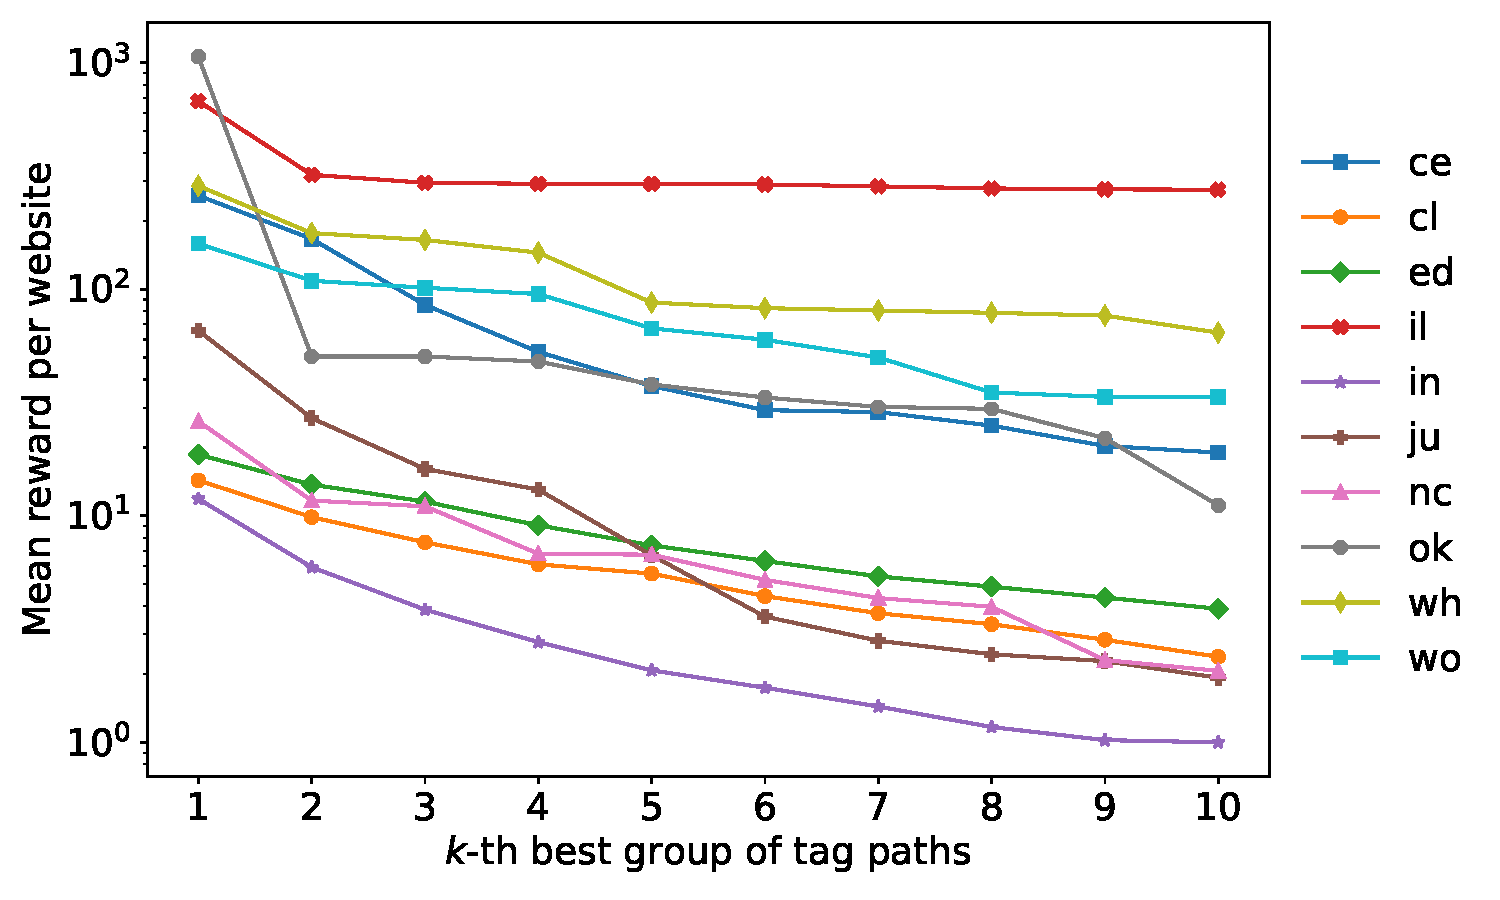
\includegraphics[width=\linewidth]{plots/top_k_dom_groups.pdf}
	\caption{Mean rewards of the top-10 groups of tag paths for the ten
  selected websites from Figure~\ref{fig:10_sites_plots} (log $y$-scale)}
	\label{fig:top_k_dom_groups}
\end{figure}

\begin{table*}
	\centering
	\caption{Mean and STD of non-zero rewards of the
  learning agent on each website}
	\begin{tabular}{ccccccccccccccccccc}
		\toprule
		               & \emph{ab} & \emph{as} & \emph{be} & \emph{ce} & \emph{cl} & \emph{cn} & \emph{ed} & \emph{il} & \emph{in} & \emph{is} & \emph{jp} & \emph{ju} & \emph{nc} & \emph{oe} & \emph{ok} & \emph{qa} & \emph{wh} & \emph{wo} \\
		\midrule
		\bfseries Mean & \01.7     & 1.5       & \04.5     & \030.2    & 12.4      & 4.2       & 2.5       & \03.1     & 1.6       & \03.5     & \03.5     & \05.4     & \02.0     & \02.5     & \05.5     & 15.4      & \03.0     & \02.1     \\
		\bfseries Std  & 16.8      & 5.35      & 20.9      & 290.3     & \02.8     & 8.9       & 7.1       & 53.9      & 4.2       & 11.1      & 17.4      & 10.5      & \08.7     & \09.3     & 13.9      & 18.8      & 22.0      & 43.5      \\
		\bottomrule
	\end{tabular}
	\label{tab:websites_rewards}
\end{table*}

We first study the reward associated by our algorithm to tag paths.
Figure~\ref{fig:top_k_dom_groups} shows the mean reward of the top 10
path groups (logarithmic $y$-axis), for the ten websites in Figure~\ref{fig:10_sites_plots}.
Top groups have high rewards: across websites, the best group averages 258, followed by 89, 74, 67, and 41 for the 10th, showing that \textbf{our SB agent effectively identifies tag path groups leading to HTML pages with target links}. Although the first group often dominates, several groups still yield substantial reward, so restricting to the top one is insufficient. Comparing Figure~\ref{fig:top_k_dom_groups} with the
mean rewards for each website (on groups with non-zero rewards)
in Table~\ref{tab:websites_rewards}, the top 10 groups
generally far exceed the overall mean
(e.g., for \emph{wo}, the the 10th group scores 33.5 v.s.\
 2.1 for the mean). This is also clear
from the high STD values from Table~\ref{tab:websites_rewards} (over 20 times the mean for \emph{wo})
implying significant differences in the rewards of different
	groups: rewards are not normally distributed across groups but more
closely resemble a power law.
Table~\ref{tab:websites_rewards} also shows large cross-website reward disparities, leading to the impossibility of setting an optimal exploration--exploitation trade-off coefficient~$\alpha$. This supports our pragmatic choice of $\alpha=2\sqrt{2}$, effective in practice. These disparities further highlight strong heterogeneity in target concentration across websites, complementing Sec.~\ref{subsection:dataset_characteristics}.

Examining top-group tag paths often reveals clues about target-rich areas. In \emph{nc}, a typical path includes \texttt{div.container.w-iap/}
\noindent\texttt{div.iap-content}, linked to the \emph{International Activities Program}, a program focused on collecting international education statistics. In \emph{wo}, paths include \texttt{collections-sief}, related to the \emph{Strategic Impact Evaluation Fund}, a trust fund producing data and reports. Some groups directly include target-retrieval keywords, e.g., \texttt{fr-link--download} in \emph{ju} or \texttt{status-publish} in \emph{ok}. Other websites' top paths are not  human-interpretable yet still achieve high rewards (examples in~\cite{github_repository}). This shows that our agent detects useful patterns even without semantic meaning, adapting to diverse structures without prior knowledge and supporting an online, per-website learning approach. 
It further demonstrates how our approach is language-independent: the RL agent learns structural patterns in HTML pages regardless of semantic meaning, enabling efficient target retrieval even on non-English or multilingual websites.

Assessing the concrete precision of our approach to retrieving SDs
requires determining the number of SDs collected in the targets.
Detecting statistics tables in heterogeneous formats is costly: even
state-of-the-art methods require roughly one second per PDF
page~\cite{soric2025benchmarkingtableextractionheterogeneous};
spreadsheets pose similar challenges~\cite{vitagliano2021detecting}.
Performing this online or at scale remains an open problem. As an empirical peak into the SD retrieval precision, we manually analyze a random sample of $7\times 40=280$ targets from 7 diverse websites in Table~\ref{tab:stats_tables}, counting the percentage of targets containing at least one statistics table (\textbf{``SD Yield''}) and their mean number per target (\textbf{``Mean \# SDs / Target''}). Results show that even on non-statistical websites (\emph{ed}, \emph{in}, \emph{oe}, \emph{wh}), an important fraction of targets contains SDs; although many targets contain none, SDs concentrate on a subset, yielding in most cases more than two SDs per collected target.

\begin{table}
	\centering
	\caption{SDs retrieval across sample targets}
	\begin{tabular}{lccccccc}
		\toprule
		& \emph{be} & \emph{ed} & \emph{is} & \emph{in} & \emph{nc} & \emph{oe} & \emph{wh} \\
		\midrule
		\bfseries SD Yield (\%) & 82 & 35 & 93 & 40 & 83 & 60 & 40 \\
		\bfseries Mean \# SDs / Target & 9.1 & 2.8 & 2.9 & 2.1 & 2.1 & 4.9 & 1.4 \\
		\bottomrule
	\end{tabular}
	\label{tab:stats_tables}
\end{table}

\begin{toappendix}
  \subsection{Effectiveness of SB Learning}

  A typical tag path containing reference to IAP in the website \emph{nc}
  is:
  \begin{quote}
    \path{/html/body/div.nces/div.container.w-iap/div.iap-content/div.row/div.col-md-6/h4/a}
  \end{quote}
  and to SIEF in the website \emph{wo}:
  \begin{quote}
  \path{/html/body/div.wp-page-body.container.default-wrapper page-collections.collections-sief/div.body-content-wrap.theme-nada-2/div.about-collection/div.repository-container/div.body/div/p/a}
  \end{quote}

  Examples of tag paths including keywords related to target retrieval are
  \begin{quote}
  \path{/html/body.path-node.page-node-type-ressource/div.dialog-off-canvas-main-canvas/div.layout-container/main#main-content/div.layout-content/div.region.region-content/div.block.block-system.block-system-main-block#block-open-theme-contenudelapageprincipale/article.mj-resource.mj-break-word.node--promoted/div.fr-container.mj-ressource__content/div.fr-grid-row.fr-grid-row--gutters.mj-content__corps/div.fr-col-lg-8.fr-col-offset-lg-2.fr-col-12.content-container__paragraph/section.fr-downloads-group.fr-downloads-group--multiple-links/ul/li/a.fr-link fr-link--download}
  \end{quote}
for \emph{ju}, and
  \begin{quote}
  \path{/html/body.home.page-template.page-template-onecolumn-page.page-template-onecolumn-page-php.page.page-id-7/main.content/div.container/div.row/div.main col-md-12/article.post.post-7.page.type-page.status-publish.hentry#post-7/div.entry-content/div#stcpDiv/div/strong/a}
  \end{quote}
for \emph{ok}.

Many other websites however have typical target-rich tag paths that cannot be interpreted by humans: for instance on \emph{jp} we have
  \begin{quote}
  \path{/html/body.top/div#wrapper/div#groval_navi/ul#groval_menu/li.menu-item-has-children/ul.sub-menu/li/a}
  \end{quote}
 on \emph{il} we have
  \begin{quote}
  \path{/html/body/div.container.s-lib-side-borders.pad-top-med#s-lg-side-nav-content/div.row/div.col-md-9/div.s-lg-tab-content/div.tab-pane.active#s-lg-guide-main/div.row.s-lg-row/div.col-md-12#s-lg-col-1/div.s-lg-col-boxes/div.s-lg-box-wrapper-17054143#s-lg-box-wrapper-17054143/div.s-lib-box-container#s-lg-box-14451639-container/div.s-lib-box.s-lib-box-std#s-lg-box-14451639/div#s-lg-box-collapse-14451639/div.s-lib-box-content/div.clearfix#s-lg-content-31285074/ul/li/a}
  \end{quote}
 and on \emph{ed} we have
  \begin{quote}
  \path{/html/body.cf-rtm/div.accueil-portail#page/div.container#main-ermes-container/main#main/div#readspeaker-container/div#portal/div.row/div.col-md-12.cms-inner-layout#layout-2/div.row/div.col-md-6.cms-inner-zone#zone-4/div#frame-224/div.frame.frame-portalcarouselwebframefactory.hidden-print/div.frame-standard.panel.panel-front.webframe-ermes-carousel/div.panel-body/div.ermes-frame-html#carousel-4AD04CE72B556A3CCF5DFCF7FB70964E/div.rsItem/div.modele_13.model-html/table/tbody/tr/td/a.vide}
  \end{quote}

\end{toappendix}

\begin{toappendix}
\subsection{URL Classification Quality}\label{subsubsection:url_classifier_results}

\begin{table}[h]
	\centering
  \vspace{-1em}
	\caption{Confusion matrix of the URL classifier, on the 11
		fully-crawled websites (average over 15 runs)}
	\vspace*{-.5em}
	\begin{tabular}{lrrr}
		\toprule
    \bfseries \diagbox{True}{Predicted} & \bfseries HTML (\%)    &
		\bfseries Target (\%)    & \bfseries Neither (\%)              \\
		\midrule
		\bfseries HTML           & 58.04                  & \01.37 & 0.00 \\
		\bfseries Target         & \00.75                 & 32.19  & 0.00 \\
		\bfseries Neither        & \05.34                 & \02.41 & 0.00 \\
		\bottomrule
	\end{tabular}
	\label{tab:cm_pcts_11_sites}
\end{table}

The confusion matrix of our URL classifier, averaged over 15 runs, for all fully-crawled websites, is presented
in Table~\ref{tab:cm_pcts_11_sites}.

We observe that classification errors are extremely marginal on ``HTML''
	and ``Target'' URLs. Never classifying as ``Neither'' leads to some
classification errors (discussed in Sec.~\ref{subsection:url_classifier}),
ultimately responsible for the difference between the number of requests 
made by
\textsf{\small SB-CLASSIFIER} and \textsf{\small SB-ORACLE} on the 11 fully-crawled websites. However, since the classifier oracle is unfeasible in
practice, the performance of
\textsf{\small SB-CLASSIFIER} is satisfactory.
\end{toappendix}

\subsection{Early-Stopping}\label{sec:early_stopping}

To prevent the crawler from continuing on websites with few or no remaining targets, we add an early-stopping mechanism. Every $\nu$ iterations, we compute a slope $\sigma = \tfrac{y_t - y_{t-\nu}}{\nu}$, representing the growth rate in the number $y_t$ of targets at crawling step~$t$. We then maintain an exponential moving average $\mu = \gamma \cdot \sigma + (1-\gamma)\cdot \mu$, with $\gamma$ the decay rate. If $\mu$ stays below a threshold $\epsilon$ for $\kappa$ consecutive slopes (i.e., $\kappa \cdot \nu$ iterations), crawling stops. Parameters ($\nu=1000$, $\epsilon=0.2$, $\gamma=0.05$, $\kappa=15$) provide a good balance between avoiding premature termination and efficiently stopping on exhausted sites.

The lower part of Table~\ref{tab:all_crawlers_all_sites_nb_requests} (below the double rule) shows early-stopping results: the percentage of requests avoided and of targets missed. High values are better for the former, low for the latter. We observe three behaviors:
\begin{inparaenum}[(i)]
  \item Medium to large websites where target discovery slows and stopping occurs effectively (\emph{ab}, \emph{ed}, \emph{in}, \emph{jp}, \emph{ju}, \emph{nc}, \emph{ok}). Smaller sites take longer (in \%) to stop due to the required $\kappa \cdot \nu$ iterations;
  \item Large websites with continuous target discovery where stopping conditions are never met before manual termination (\emph{as}, \emph{ce}, \emph{il}, \emph{oe}, \emph{wh}, \emph{wo});
	\item Small sites (\emph{be}, \emph{cl}, \emph{cn}, \emph{qa}) where the crawl ends before early stopping can trigger within $\kappa \cdot \nu = 15$k iterations; this is not an issue, as these sites are quickly fully crawled.
\end{inparaenum}

\begin{toappendix}
  \subsection{Early-Stopping}
  \begin{figure}[h]
	\begin{subfigure}[t]{0.49\linewidth}
		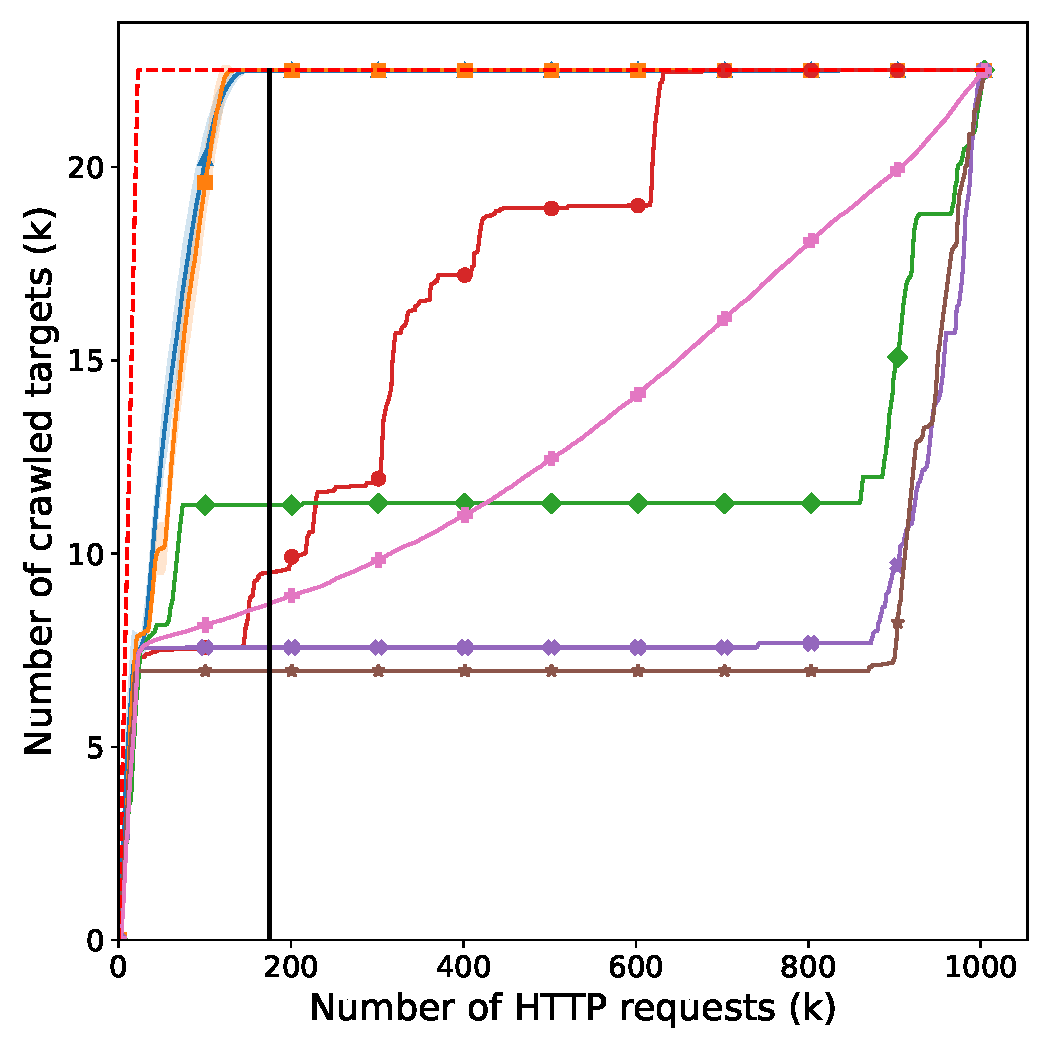
\includegraphics[width=\linewidth]{plots/early_stopping/in.pdf}

		\vspace{-1em}
		\caption{\emph{in}}
		\label{fig:in_early_stopping}
	\end{subfigure}
	\begin{subfigure}[t]{0.49\linewidth}
		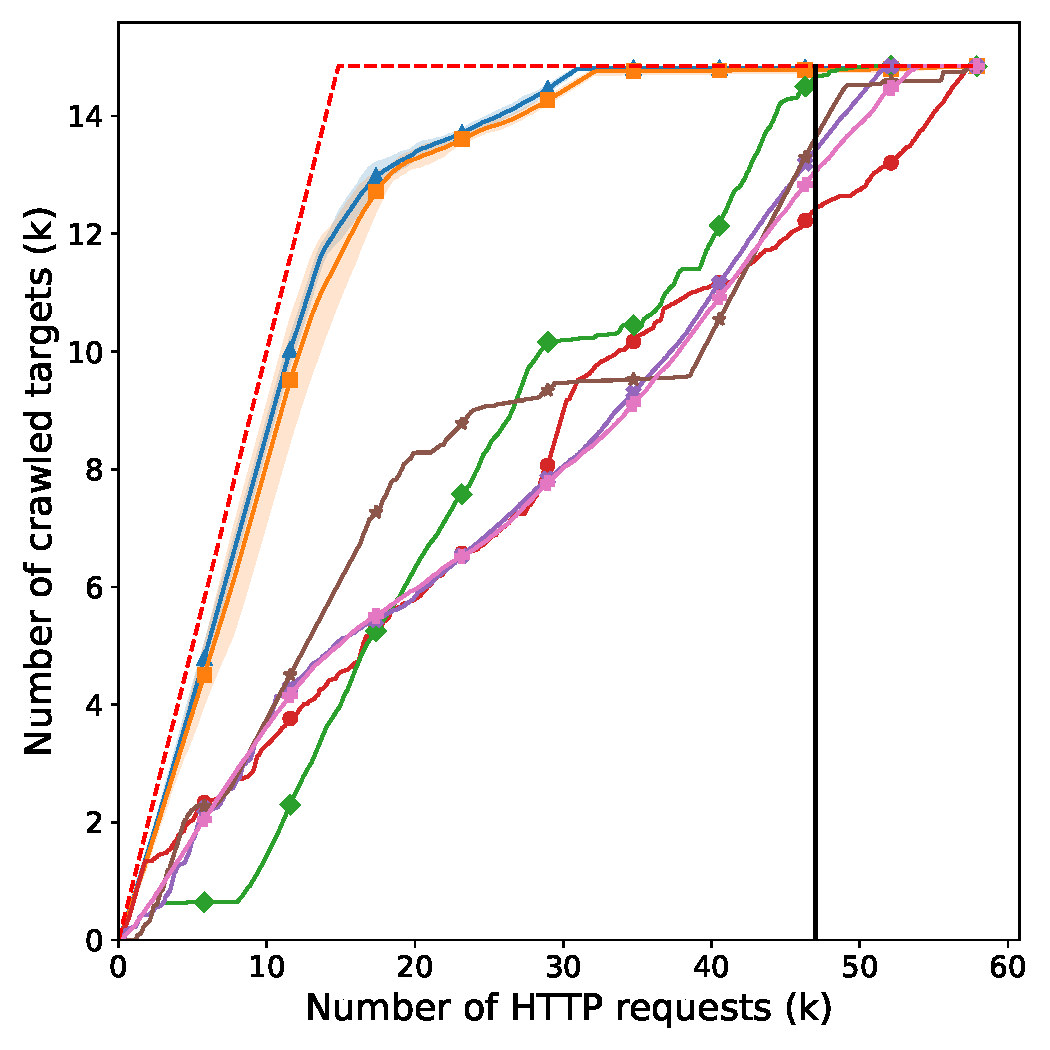
\includegraphics[width=\linewidth]{plots/early_stopping/ju.pdf}

		\vspace{-1em}
		\caption{\emph{ju}}
		\label{fig:ju_early_stopping}
	\end{subfigure}
	\vspace{-.75em}
	\caption{Visualization of early-stopping time (black rule) for websites \emph{in} and \emph{ju}}
	\label{fig:early_stopping_in_ju}
\end{figure}

	Figure~\ref{fig:early_stopping_in_ju} presents a visualization of
  the early-stopping mechanism applied to two websites: \emph{in} and
\emph{ju} (right). Both fall under the first behavior described in
Sec.~\ref{sec:early_stopping}, illustrating that smaller websites take
longer (in \%) to stop after the first signs of target convergence. For
\emph{in}, stopping occurs shortly after the point where a human would
likely have cut, but for \emph{ju}, the delay is more important. Despite
early signs of convergence, stopping is postponed due to the fixed
$\kappa \cdot \nu =15\,000$ threshold, which represents a much larger fraction of the site for \emph{ju} (60k pages) than for \emph{in} (1M pages).

\bigskip
\end{toappendix}

\begin{comment}
\begin{table}
	\centering
	\caption{Confusion matrix of the URL classifier used in the SB algorithm on website \emph{be} (on average, for 15 runs).}
	\begin{tabular}{lrrr}
		\toprule
		\bfseries True/Predicted & \bfseries HTML & \bfseries Target & \bfseries Neither \\
		\midrule
		\bfseries HTML           & 11231          & \0\0272          & \0\0\0\00         \\
		\bfseries Target         & \0\0732        & 15321            & \0\0\0\00         \\
		\bfseries Neither        & \02436         & \02296           & \0\0\0\00         \\
		\bottomrule
	\end{tabular}
	\label{tab:cm_be}
\end{table}

% 34.784  0.842 0
% 2.267 47.451 0
% 7.545 7.111 0

\begin{table}
	\centering
	\caption{Confusion matrix of the URL classifier used in the SB algorithm on website \emph{cl} (on average, for 15 runs).}
	\begin{tabular}{lrrr}
		\toprule
		\bfseries True/Predicted & \bfseries HTML & \bfseries Target & \bfseries Neither \\
		\midrule
		\bfseries HTML           & 1654           & \0\024           & \0\0\00           \\
		\bfseries Target         & \0154          & 3538             & \0\0\00           \\
		\bfseries Neither        & \0104          & \0340            & \0\0\00           \\
		\bottomrule
	\end{tabular}
	\label{tab:cm_cl}
\end{table}

% 28.449 4.128 0
% 2.649 60.853 0
% 3.696  5.848 0

\begin{table}
	\centering
	\caption{Confusion matrix of the URL classifier used in the SB algorithm on website \emph{cn} (on average, for 15 runs).}
	\begin{tabular}{lrrr}
		\toprule
		\bfseries True/Predicted & \bfseries HTML & \bfseries Target & \bfseries Neither \\
		\midrule
		\bfseries HTML           & 5272           & \0\0\07          & \0\0\00           \\
		\bfseries Target         & \0\064         & 7423             & \0\0\00           \\
		\bfseries Neither        & \0\0\08        & \0\016           & \0\0\00           \\
		\bottomrule
	\end{tabular}
	\label{tab:cm_cn}
\end{table}

% 41.220 0.055 0
% 0.500 58.038 0
% 0.063 0.125 0

\begin{table}
	\centering
	\caption{Confusion matrix of the URL classifier used in the SB algorithm on website \emph{ed} (on average, for 15 runs).}
	\begin{tabular}{lrrr}
		\toprule
		\bfseries True/Predicted & \bfseries HTML & \bfseries Target & \bfseries Neither \\
		\midrule
		\bfseries HTML           & 85920          & \02610           & \0\0\0\0\00       \\
		\bfseries Target         & \0\0175        & 10180            & \0\0\0\0\00       \\
		\bfseries Neither        & \08645         & \01348           & \0\0\0\0\00       \\
		\bottomrule
	\end{tabular}
	\label{tab:cm_ed}
\end{table}

% 78.914 2.397 0
% 0.160 9.350 0
% 7.940 1.238 0

\begin{table}
	\centering
	\caption{Confusion matrix of the URL classifier used in the SB algorithm on website \emph{in} (on average, for 15 runs).}
	\begin{tabular}{lrrr}
		\toprule
		\bfseries True/Predicted & \bfseries HTML & \bfseries Target & \bfseries Neither \\
		\midrule
		\bfseries HTML           & 883706         & \0\0\0164        & \0\0\0\0\00       \\
		\bfseries Target         & \0\0\0117      & \022362          & \0\0\0\0\00       \\
		\bfseries Neither        & \092544        & \0\03922         & \0\0\0\0\00       \\
		\bottomrule
	\end{tabular}
	\label{tab:cm_in}
\end{table}

% 88.123 0.016 0
% 0.012 2.230 0
% 9.228 0.391 0

\begin{table}
	\centering
	\caption{Confusion matrix of the URL classifier used in the SB algorithm on website \emph{is} (on average, for 15 runs).}
	\begin{tabular}{lrrr}
		\toprule
		\bfseries True/Predicted & \bfseries HTML & \bfseries Target & \bfseries Neither \\
		\midrule
		\bfseries HTML           & 118805         & \0\0\0113        & \0\0\0\0\00       \\
		\bfseries Target         & \0\0\0120      & 168762           & \0\0\0\0\00       \\
		\bfseries Neither        & \0\01185       & \0\02292         & \0\0\0\0\00       \\
		\bottomrule
	\end{tabular}
	\label{tab:cm_is}
\end{table}

% 40.788 0.039 0
% 0.041 57.939 0
% 0.407 0.787 0

\begin{table}
	\centering
	\caption{Confusion matrix of the URL classifier used in the SB algorithm on website \emph{ju} (on average, for 15 runs).}
	\vspace{-.5em}
	\begin{tabular}{lrrr}
		\toprule
		\bfseries True/Predicted & \bfseries HTML & \bfseries Target & \bfseries Neither \\
		\midrule
		\bfseries HTML           & 40657          & \0\0143          & \0\0\0\0\00       \\
		\bfseries Target         & \0\0134        & 14711            & \0\0\0\0\00       \\
		\bfseries Neither        & \0\0404        & \01045           & \0\0\0\0\00       \\
		\bottomrule
	\end{tabular}
	\label{tab:cm_ju}
\end{table}

% 71.211 0.250 0
% 0.235 25.676 0
% 0.708 1.830 0

\begin{table}
	\centering
	\caption{Confusion matrix of the URL classifier used in the SB algorithm on website \emph{nc} (on average, for 15 runs).}
	\vspace{-.5em}
	\begin{tabular}{lrrr}
		\toprule
		\bfseries True/Predicted & \bfseries HTML & \bfseries Target & \bfseries Neither \\
		\midrule
		\bfseries HTML           & 217531         & \02193           & \0\0\0\0\00       \\
		\bfseries Target         & \0\0\0839      & 82187            & \0\0\0\0\00       \\
		\bfseries Neither        & \0\03033       & \01222           & \0\0\0\0\00       \\
		\bottomrule
	\end{tabular}
	\label{tab:cm_nc}
\end{table}

% 70.856 0.714 0
% 0.273 26.771 0
% 0.988 0.398 0

\begin{table}
	\centering
	\caption{Confusion matrix of the URL classifier used in the SB algorithm on website \emph{oe} (on average, for 15 runs).}
	\vspace{-.5em}
	\begin{tabular}{lrrr}
		\toprule
		\bfseries True/Predicted & \bfseries HTML & \bfseries Target & \bfseries Neither \\
		\midrule
		\bfseries HTML           & 143412         & 11071            & \0\0\0\0\00       \\
		\bfseries Target         & \0\01046       & 42150            & \0\0\0\0\00       \\
		\bfseries Neither        & \0\03427       & \09994           & \0\0\0\0\00       \\
		\bottomrule
	\end{tabular}
	\label{tab:cm_oe}
\end{table}

% 67.936 5.244 0
% 0.495  19.967 0
% 1.623 4.734 0

\begin{table}
	\centering
	\caption{Confusion matrix of the URL classifier used in the SB algorithm on website \emph{ok} (on average, for 15 runs).}
	\vspace{-.5em}
	\begin{tabular}{lrrr}
		\toprule
		\bfseries True/Predicted & \bfseries HTML & \bfseries Target & \bfseries Neither \\
		\midrule
		\bfseries HTML           & 391802         & \03556           & \0\0\0\0\00       \\
		\bfseries Target         & \0\0\0669      & 12058            & \0\0\0\0\00       \\
		\bfseries Neither        & \012484        & \02206           & \0\0\0\0\00       \\
		\bottomrule
	\end{tabular}
	\label{tab:cm_ok}
\end{table}

% 422775
% 92.674 0.841 0
% 0.158  2.852 0
% 2.953 0.522 0

\begin{table}
	\centering
	\caption{Confusion matrix of the URL classifier used in the SB algorithm on website \emph{qa} (on average, for 15 runs).}
	\begin{tabular}{lrrr}
		\toprule
		\bfseries True/Predicted & \bfseries HTML & \bfseries Target & \bfseries Neither \\
		\midrule
		\bfseries HTML           & 1311           & \0\031           & \0\0\00           \\
		\bfseries Target         & \0\077         & 2356             & \0\0\00           \\
		\bfseries Neither        & 1320           & \0247            & \0\0\00           \\
		\bottomrule
	\end{tabular}
	\label{tab:cm_qa}
\end{table}

% 24.541 0.580 0
% 1.441 44.103 0
% 24.71 4.624 0
\end{comment}
